
\chapter{变换矩阵}
\label{chap07}

线性代数可以用来表达许多操作,包括在三维场景中排列物体、用摄像机查看物体,以及将场景投影到屏幕上。旋转、平移、缩放和投影等几何变换可以用矩阵乘法来完成,本章的主题就是可以完成这些变换的矩阵。

如果一个点集被表示为从原点出发的偏移向量,我们将展示这些点是如何转换的,我们将用图\ref{fig:7.1}中的时钟作为一个点集的例子。因此,可以把时钟看成是一群点,它们是尾部在原点的向量的两端。我们还讨论了这些变换对位置(点)、位移向量和表面法向量的不同操作。

\section{二维线性变换(2D Linear Transformations)}

我们可以使用一个$2 \times 2$的矩阵来改变或者变换一个二维向量:

\begin{equation}
	\left[\begin{array}{ll}
		a_{11} & a_{12} \\
		a_{21} & a_{22}
	\end{array}\right]\left[\begin{array}{l}
		x \\
		y
	\end{array}\right]=\left[\begin{array}{l}
		a_{11} x+a_{12} y \\
		a_{21} x+a_{22} y
	\end{array}\right]
\nonumber
\end{equation}

这种通过简单矩阵乘法将一个二维向量与另一个二维向量相乘的操作,称为线性变换。通过这个简单的公式,我们可以实现各种有用的转换,这取决于我们在矩阵中放置的内容,这将在下面的章节中讨论。为了方便,考虑沿x轴移动是水平移动,沿y轴移动是垂直移动。

\subsection{缩放(Scaling)}

最基本的变换是沿坐标轴的缩放。该变换可以改变长度和方向:

\begin{equation}
	\operatorname{scale}\left(s_x, s_y\right)=\left[\begin{array}{cc}
		s_x & 0 \\
		0 & s_y
	\end{array}\right]
\nonumber
\end{equation}

注意到此矩阵对具有笛卡尔分量的向量$(x,y)$的作用:

\begin{equation}
	\left[\begin{array}{cc}
		s_x & 0 \\
		0 & s_y
	\end{array}\right]\left[\begin{array}{l}
		x \\
		y
	\end{array}\right]=\left[\begin{array}{l}
		s_x x \\
		s_y y
	\end{array}\right]
\nonumber
\end{equation}

因此,仅仅通过观察一个轴对齐的缩放矩阵,我们就可以读出两个缩放系数。

\begin{example}
	将x和y均匀缩小2倍的矩阵是(图\ref{fig:7.1}):
	
	\begin{equation}
		\operatorname{scale}\left(0.5, 0.5 \right)=\left[\begin{array}{cc}
			0.5 & 0 \\
			0 & 0.5
		\end{array}\right]
		\nonumber
	\end{equation}

\begin{figure}[htbp]
	\centering
	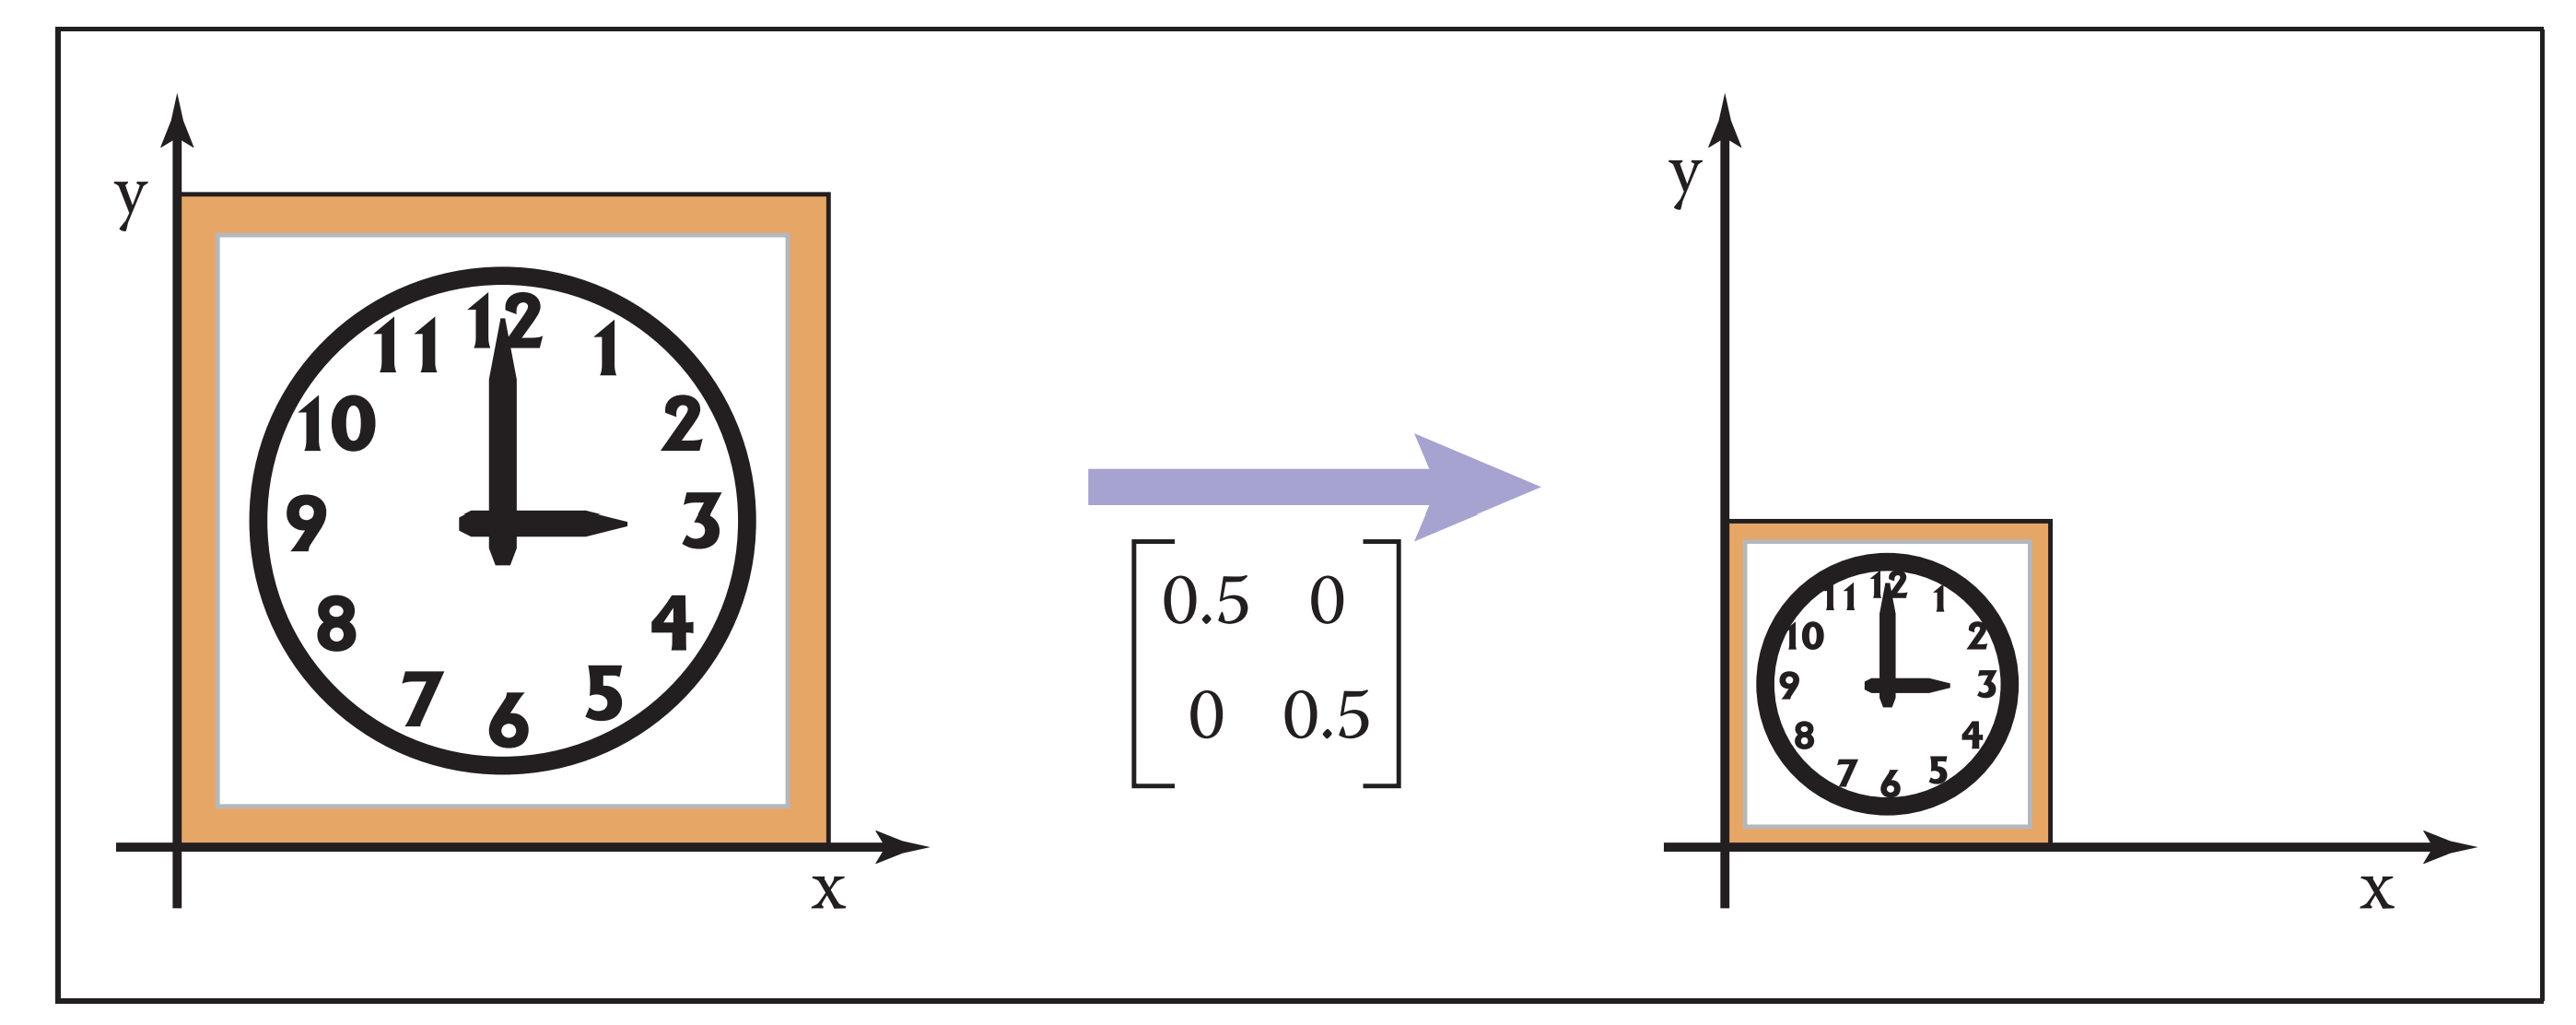
\includegraphics[scale=0.4]{Figure7.1.png}
	\caption{每个轴均匀缩放一半:轴对齐的缩放矩阵,对角线元素是缩放比例,非对角线的元素是零。}
	\label{fig:7.1}
\end{figure}

水平方向减半,垂直方向增加三倍的矩阵为(图\ref{fig:7.2}):

	\begin{equation}
		\operatorname{scale}\left(0.5, 1.5 \right)=\left[\begin{array}{cc}
			0.5 & 0 \\
			0 & 1.5
		\end{array}\right]
		\nonumber
	\end{equation}

\begin{figure}[htbp]
	\centering
	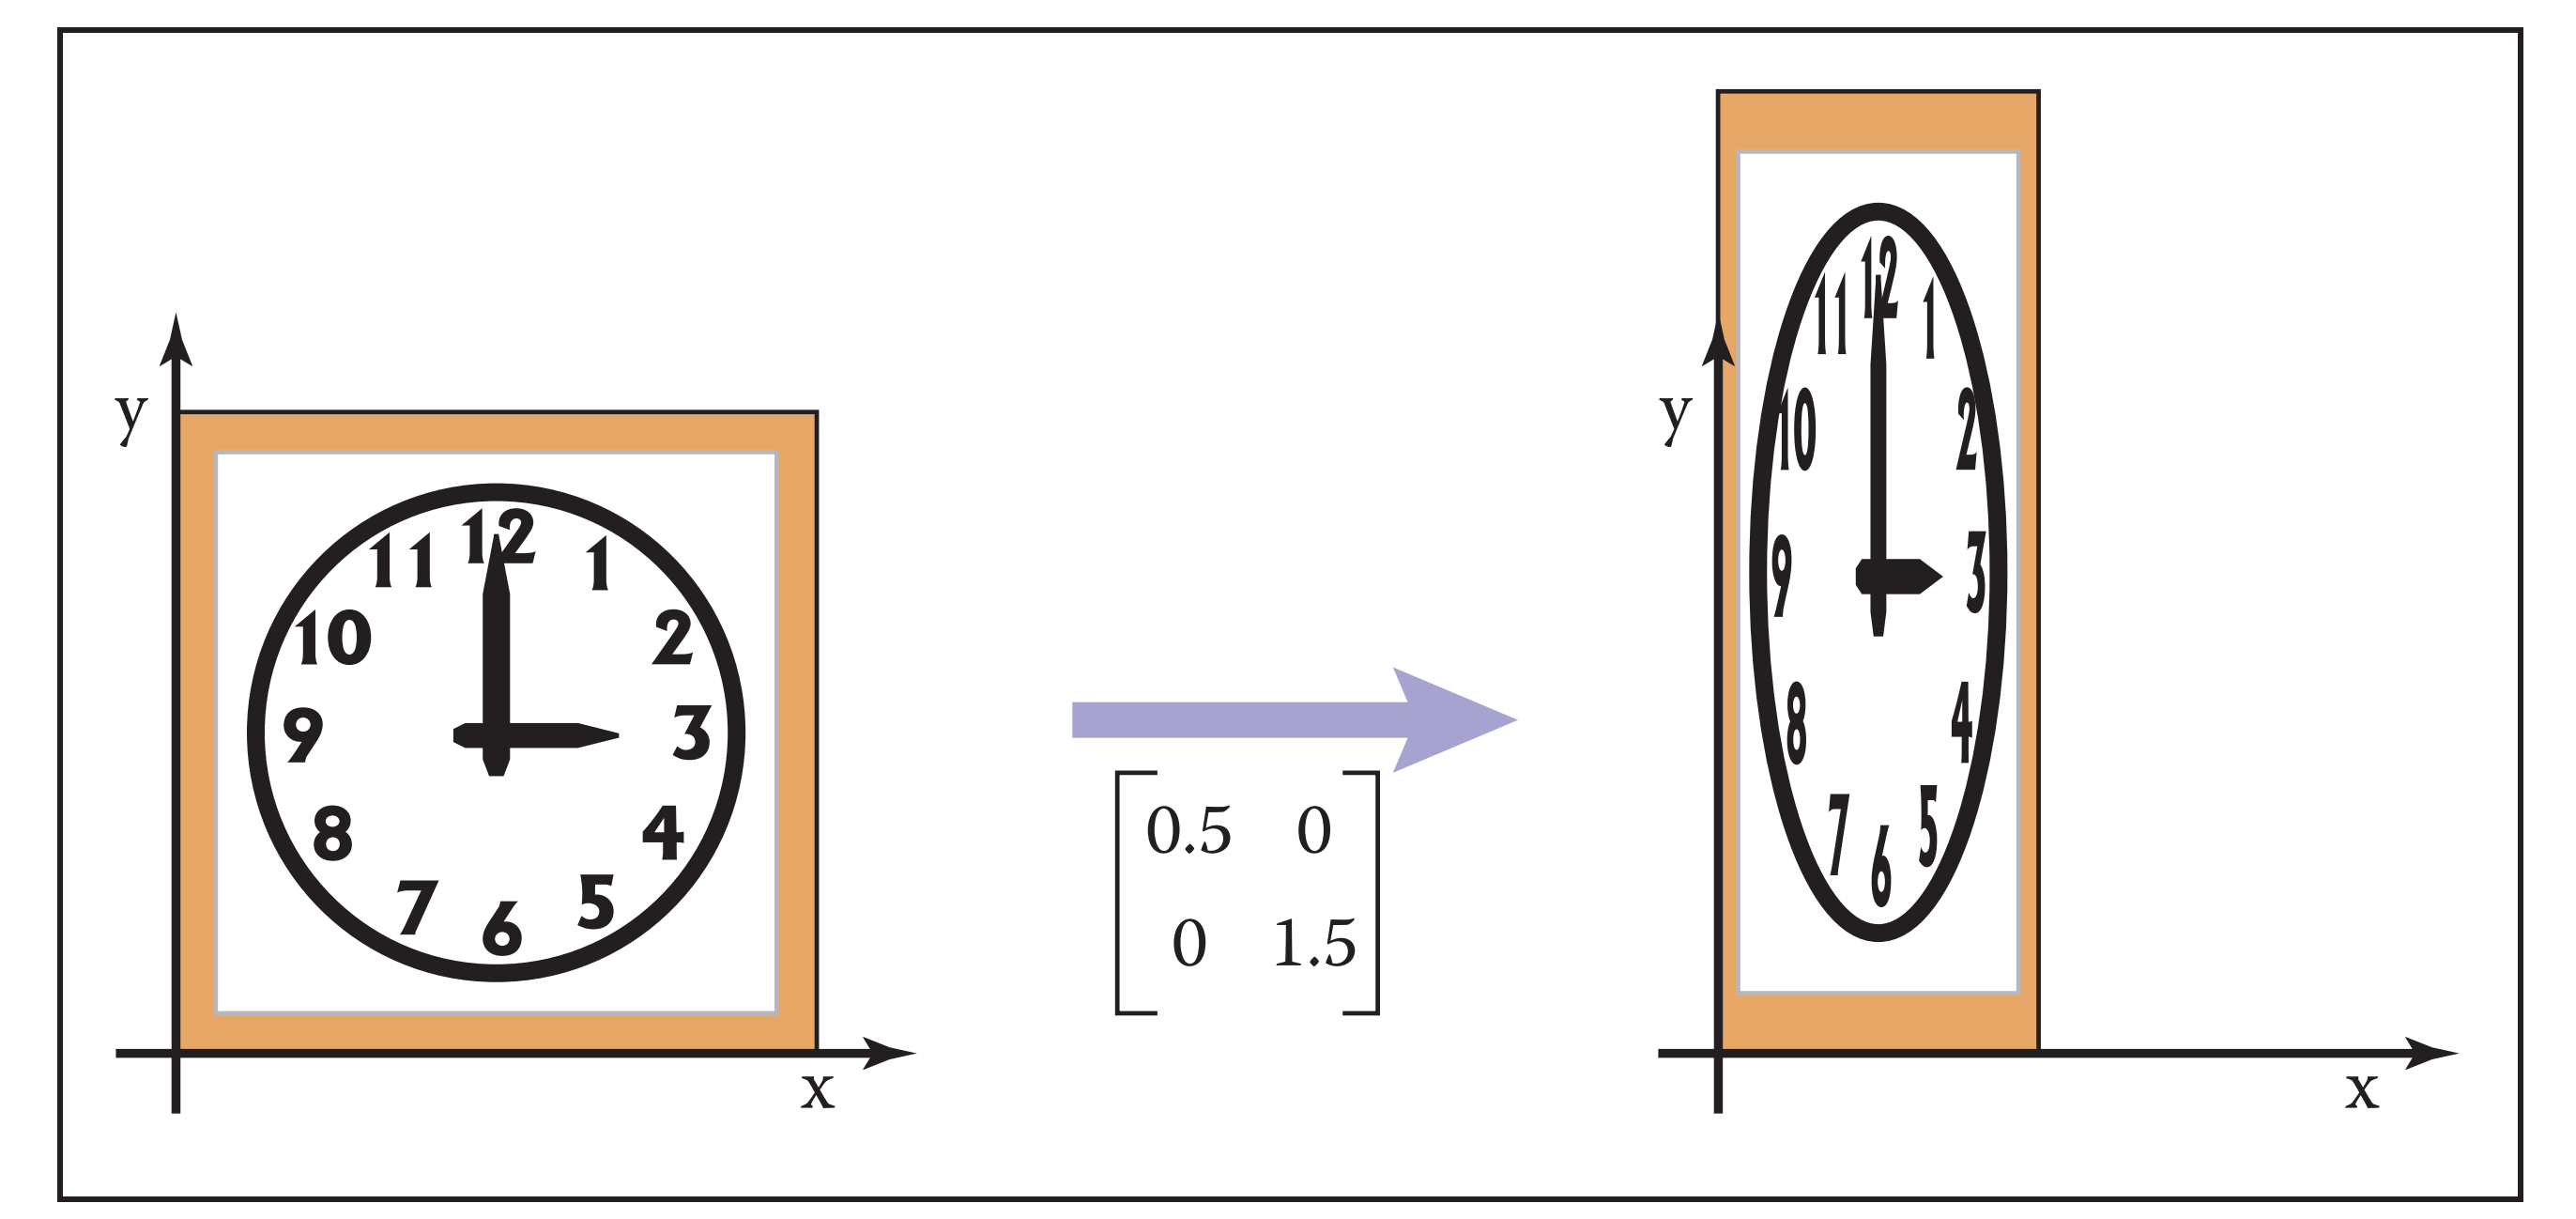
\includegraphics[scale=0.41]{Figure7.2.png}
	\caption{在x和y中不均匀缩放:缩放矩阵是对角阵,对角线元素不相等。注意到时钟的方形轮廓变为矩形,圆形则变为椭圆形。}
	\label{fig:7.2}
\end{figure}

\end{example}

\subsection{错切(Shearing)}

错切是一种将东西推向侧边,产生一种“摊牌”的效果。最下面的牌保持不动,牌越靠近牌顶,移动得越多。水平和垂直的错切矩阵是:

\begin{equation}
	\operatorname{shear-x}(s)=\left[\begin{array}{ll}
		1 & s \\
		0 & 1
	\end{array}\right], \quad \text { shear-y }(s)=\left[\begin{array}{ll}
		1 & 0 \\
		s & 1
	\end{array}\right]
\nonumber
\end{equation}

\begin{example}
	水平错切使垂直线变成向右倾斜45度线的变换是(如图\ref{fig:7.3}):
	\begin{equation}
		\operatorname{shear-x}(1)=\left[\begin{array}{ll}
			1 & 1 \\
			0 & 1
		\end{array}\right]
		\nonumber
	\end{equation}

\begin{figure}[htbp]
	\centering
	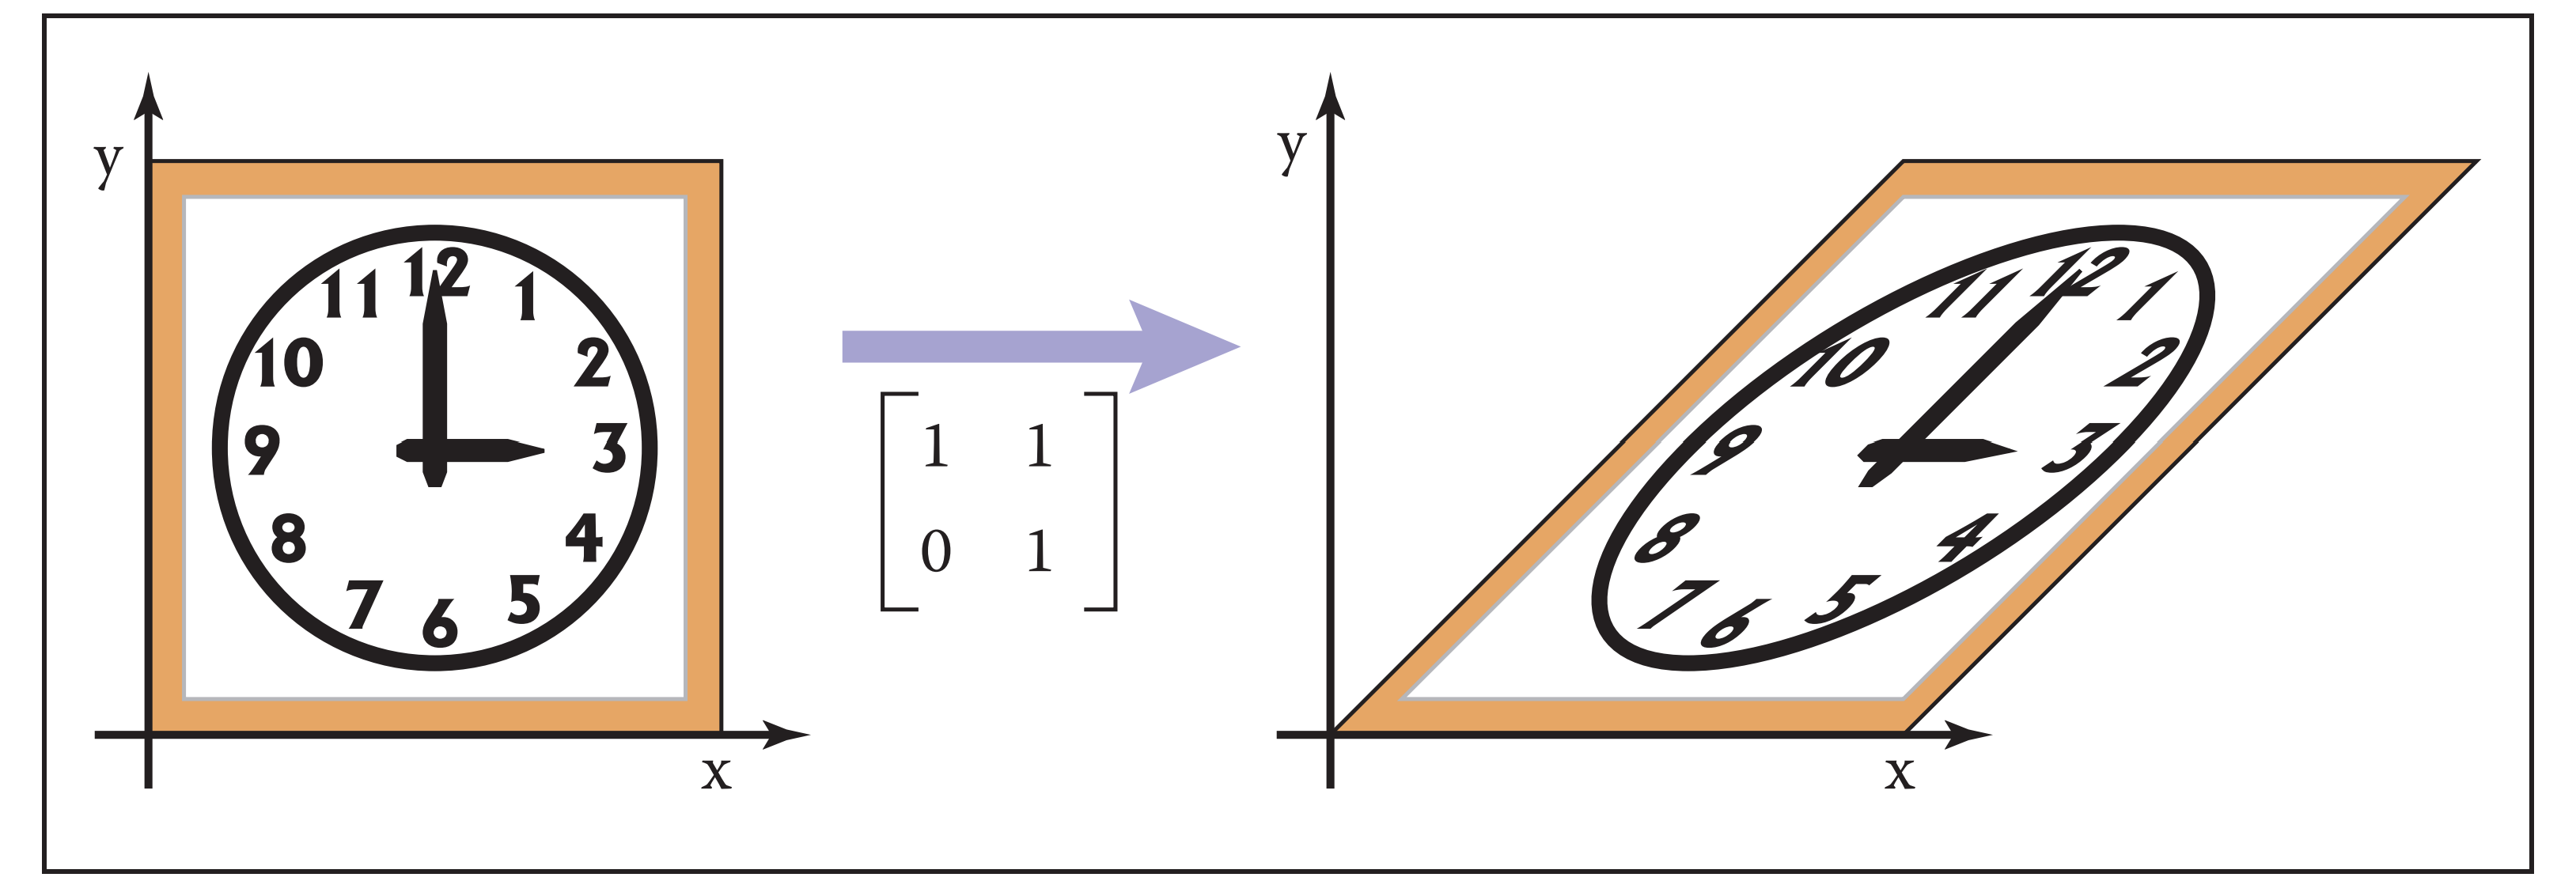
\includegraphics[scale=0.4]{Figure7.3.png}
	\caption{x错切矩阵将点向右移动,按点在y坐标位置的比例。如此,时钟的正方形轮廓变成了平行四边形,而随着缩放,时钟的圆形表面变成了椭圆。}
	\label{fig:7.3}
\end{figure}
	
\begin{figure}[htbp]
	\centering
	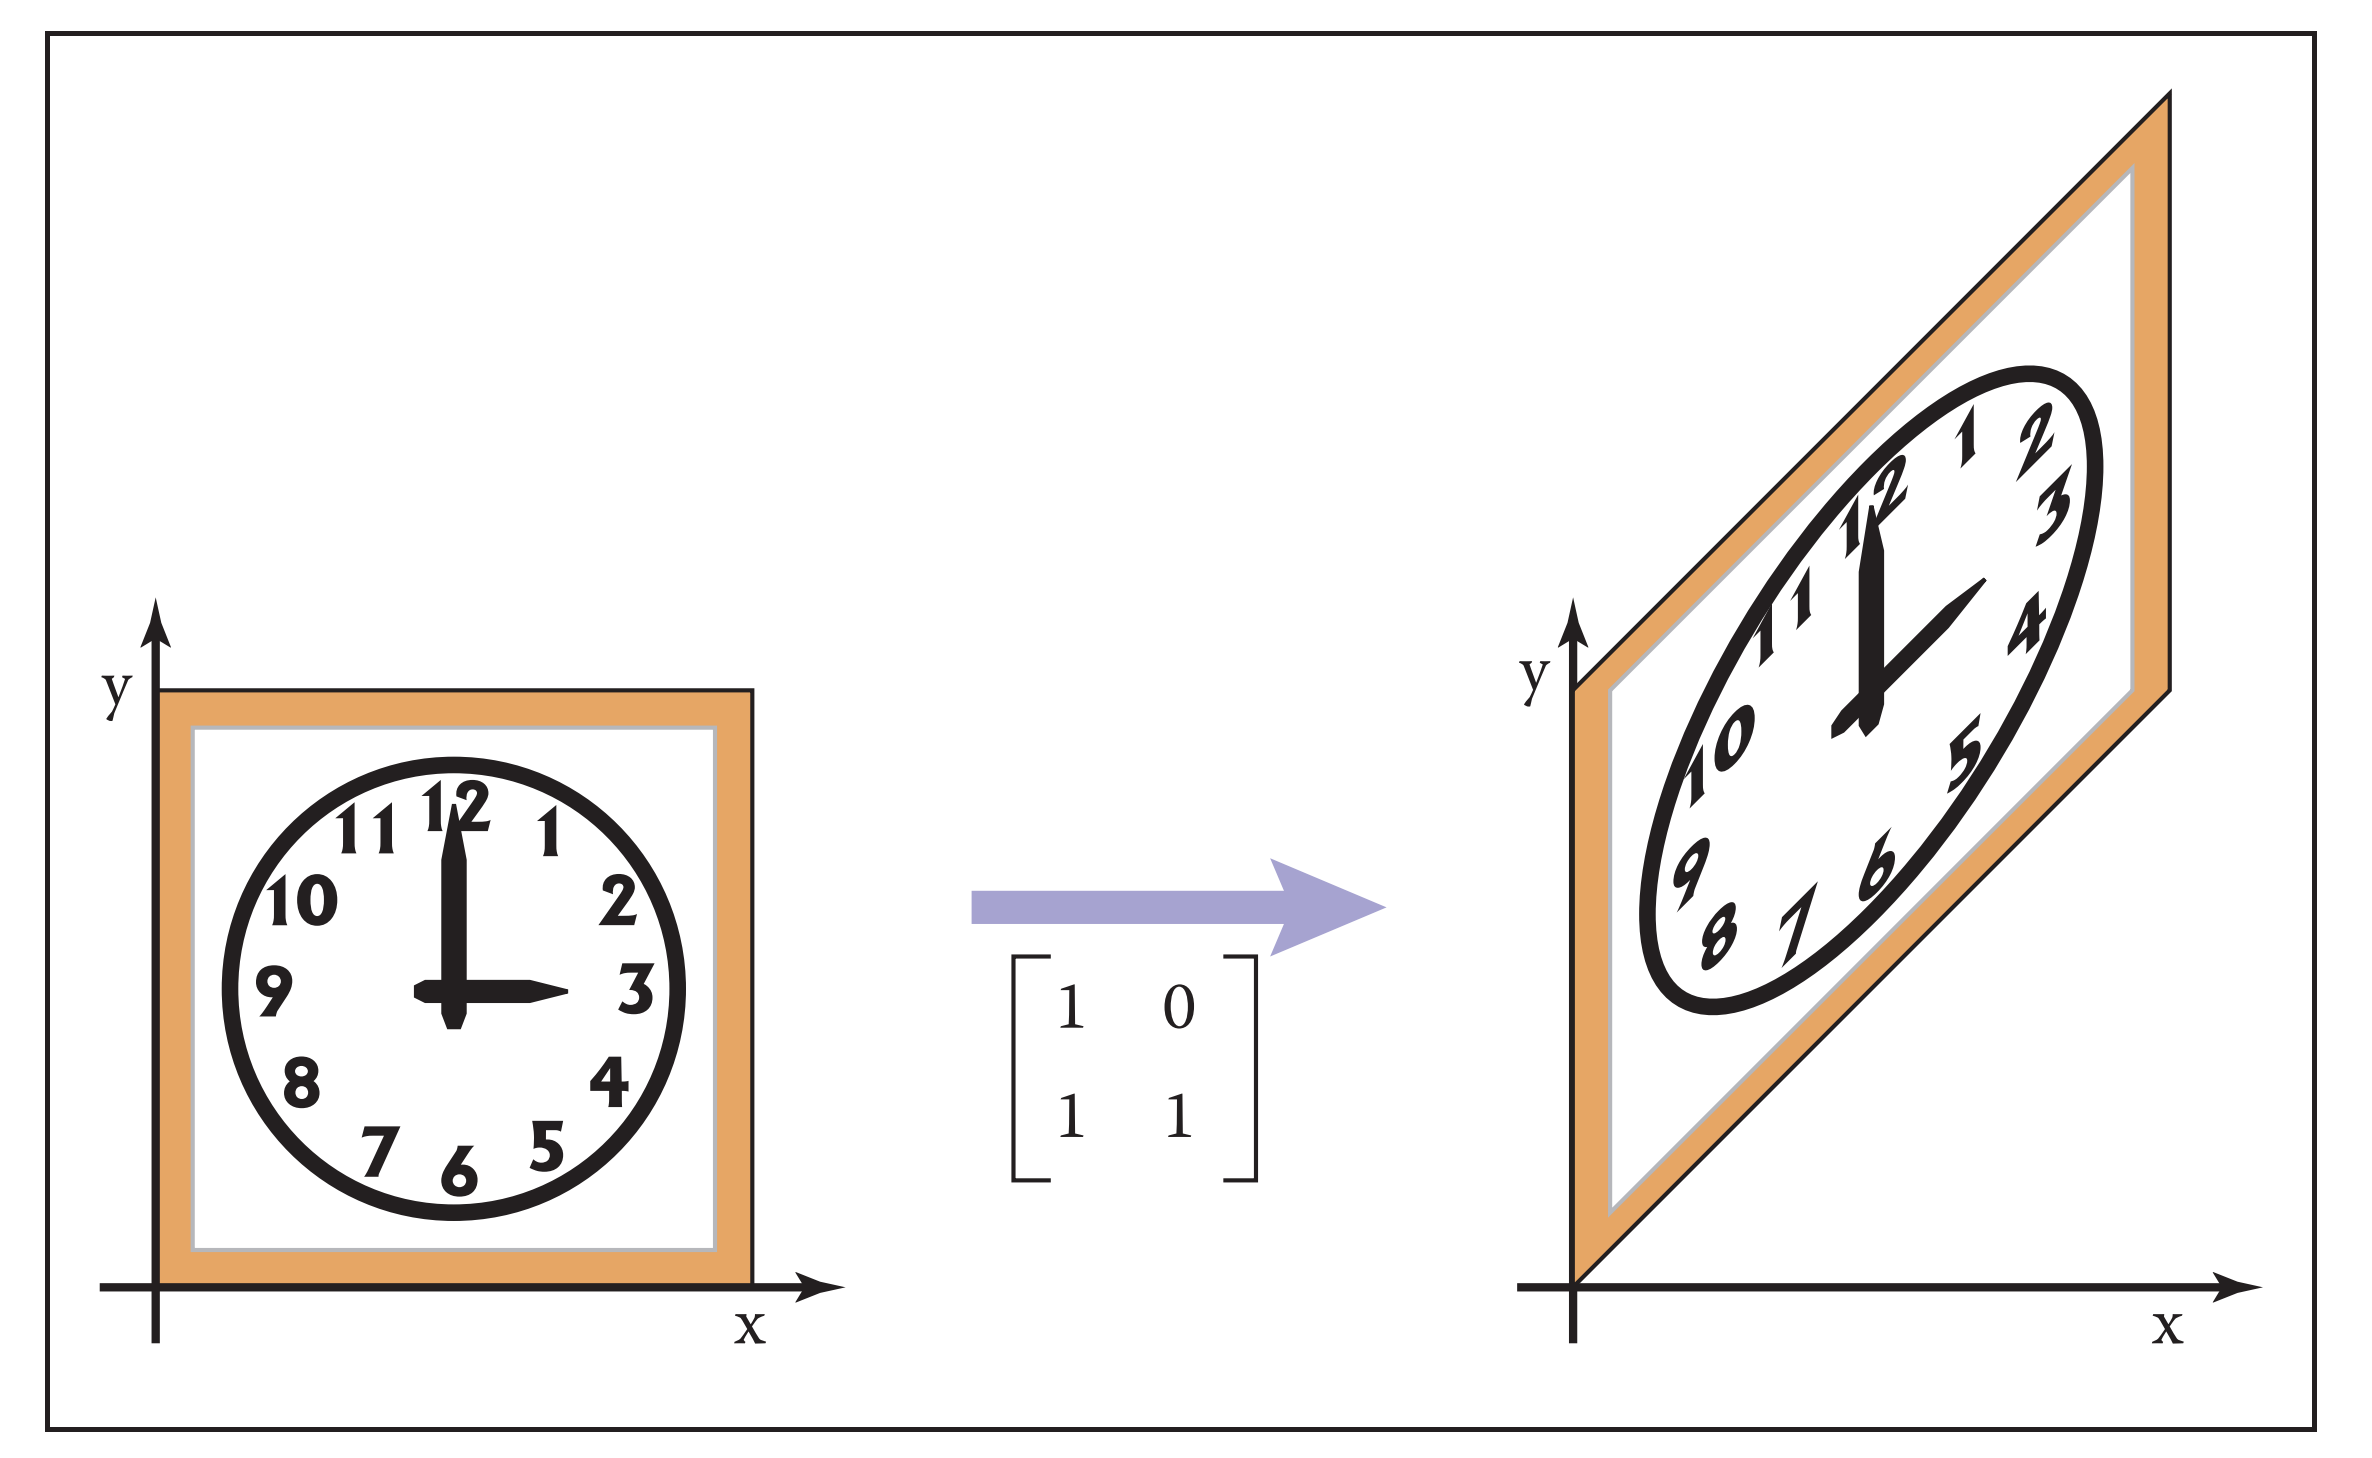
\includegraphics[scale=0.5]{Figure7.4.png}
	\caption{y错切矩阵将点向上移动,按照点在x坐标位置的比例。}
	\label{fig:7.4}
\end{figure}	
	
	垂直方向上类似的变换是(如图\ref{fig:7.4}):
	
	\begin{equation}
		\operatorname{shear-y}(1)=\left[\begin{array}{ll}
			1 & 0 \\
			1 & 1
		\end{array}\right]
		\nonumber
	\end{equation}
	
	在这两种情况下,时钟的正方形轮廓变成平行四边形,而时钟的圆形表盘外轮廓变成椭圆形\footnote{事实上,任何矩阵变换下的圆的图像都是椭圆。}。
	
	另一种考虑错切的方式是仅考虑垂直(或水平)轴的旋转。取垂直轴并顺时针倾斜角度$\phi$的错切变换为:
	
	\begin{equation}
		\left[\begin{array}{ll}
			1 &  \rm tan \phi \\
			0 & 1
		\end{array}\right]
		\nonumber
	\end{equation}

	类似地,将水平轴逆时针旋转角度$\phi$的错切矩阵为:
	
	\begin{equation}
		\left[\begin{array}{ll}
			1 &  0 \\
			\rm tan \phi & 1
		\end{array}\right]
		\nonumber
	\end{equation}
	
\end{example}

\subsection{旋转(Rotation)}

假设我们想逆时针旋转向量$\mathbf{a}$一个角度$\phi$,得到向量$\mathbf{b}$(如图\ref{fig:7.5})。如果$\mathbf{a}$与$x$轴成角度$\alpha$,其长度为$r=\sqrt{x_a^2+y_a^2}$,那么我们知道:

\begin{equation}
	\begin{aligned}
		& x_a=r \cos \alpha \\
		& y_a=r \sin \alpha
	\end{aligned}
\nonumber
\end{equation}

\begin{figure}[htbp]
	\centering
	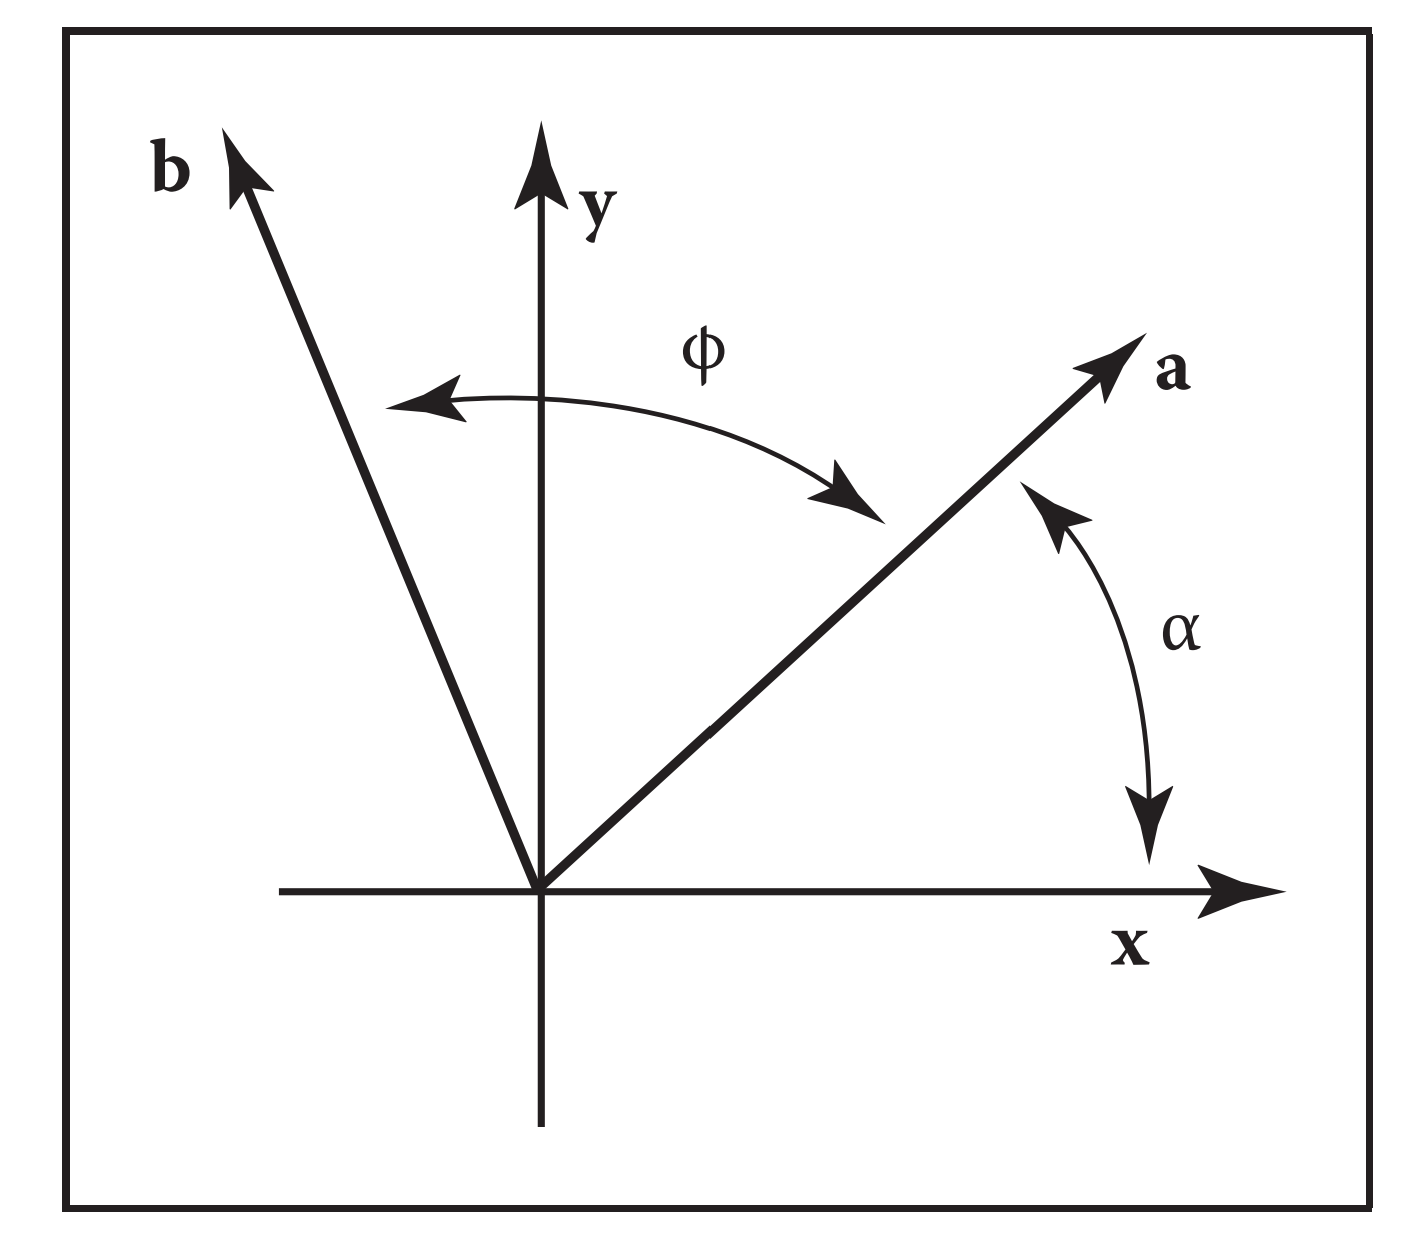
\includegraphics[scale=0.4]{Figure7.5.png}
	\caption{方程\ref{con:7.1}的几何图示}
	\label{fig:7.5}
\end{figure}	

因为$\mathbf{b}$是$\mathbf{a}$旋转而来,所以$\mathbf{b}$的长度也是$r$。$\mathbf{b}$是$\mathbf{a}$旋转$\phi$角度,所以$\mathbf{b}$与$x$轴之间的夹角是$(\alpha + \phi)$。使用三角加法恒等式(第\ref{label}小节):

\begin{equation}\label{con:7.1}
	\begin{aligned}
		& x_b=r \cos (\alpha+\phi)= r \cos \alpha \cos \phi-r \sin \alpha \sin \phi \\
		& y_b=r \sin (\alpha+\phi)= r \sin \alpha \cos \phi+r \cos \alpha \sin \phi
	\end{aligned}
\end{equation}

将$\mathbf{a}$向量带入式\ref{con:7.1},$x_a=r \cos \alpha$,$y_a=r \sin \alpha$,故可以得到:

\begin{equation}
	\begin{aligned}
		 x_b &= x_a \cos \phi - y_a \sin \phi \\
		 y_b &= y_a \cos \phi + x_a \sin \phi
	\end{aligned}
\nonumber
\end{equation}

所以从$\mathbf{a}$变换到$\mathbf{b}$的矩阵形式为:

\begin{equation}
	\operatorname{rotate}(\phi)=\left[\begin{array}{rr}
		\cos \phi & -\sin \phi \\
		\sin \phi & \cos \phi
	\end{array}\right]
\nonumber
\end{equation}

\begin{example}
	旋转$pi / 4$弧度($45^{\circ}$)的旋转矩阵是(如图\ref{fig:7.6}):
	\begin{equation}
		\left[\begin{array}{cr}
			\cos \frac{\pi}{4} & -\sin \frac{\pi}{4} \\
			\sin \frac{\pi}{4} & \cos \frac{\pi}{4}
		\end{array}\right]=\left[\begin{array}{rr}
			0.707 & -0.707 \\
			0.707 & 0.707
		\end{array}\right] \text {. }
	\end{equation}
	
	\begin{figure}[htbp]
		\centering
		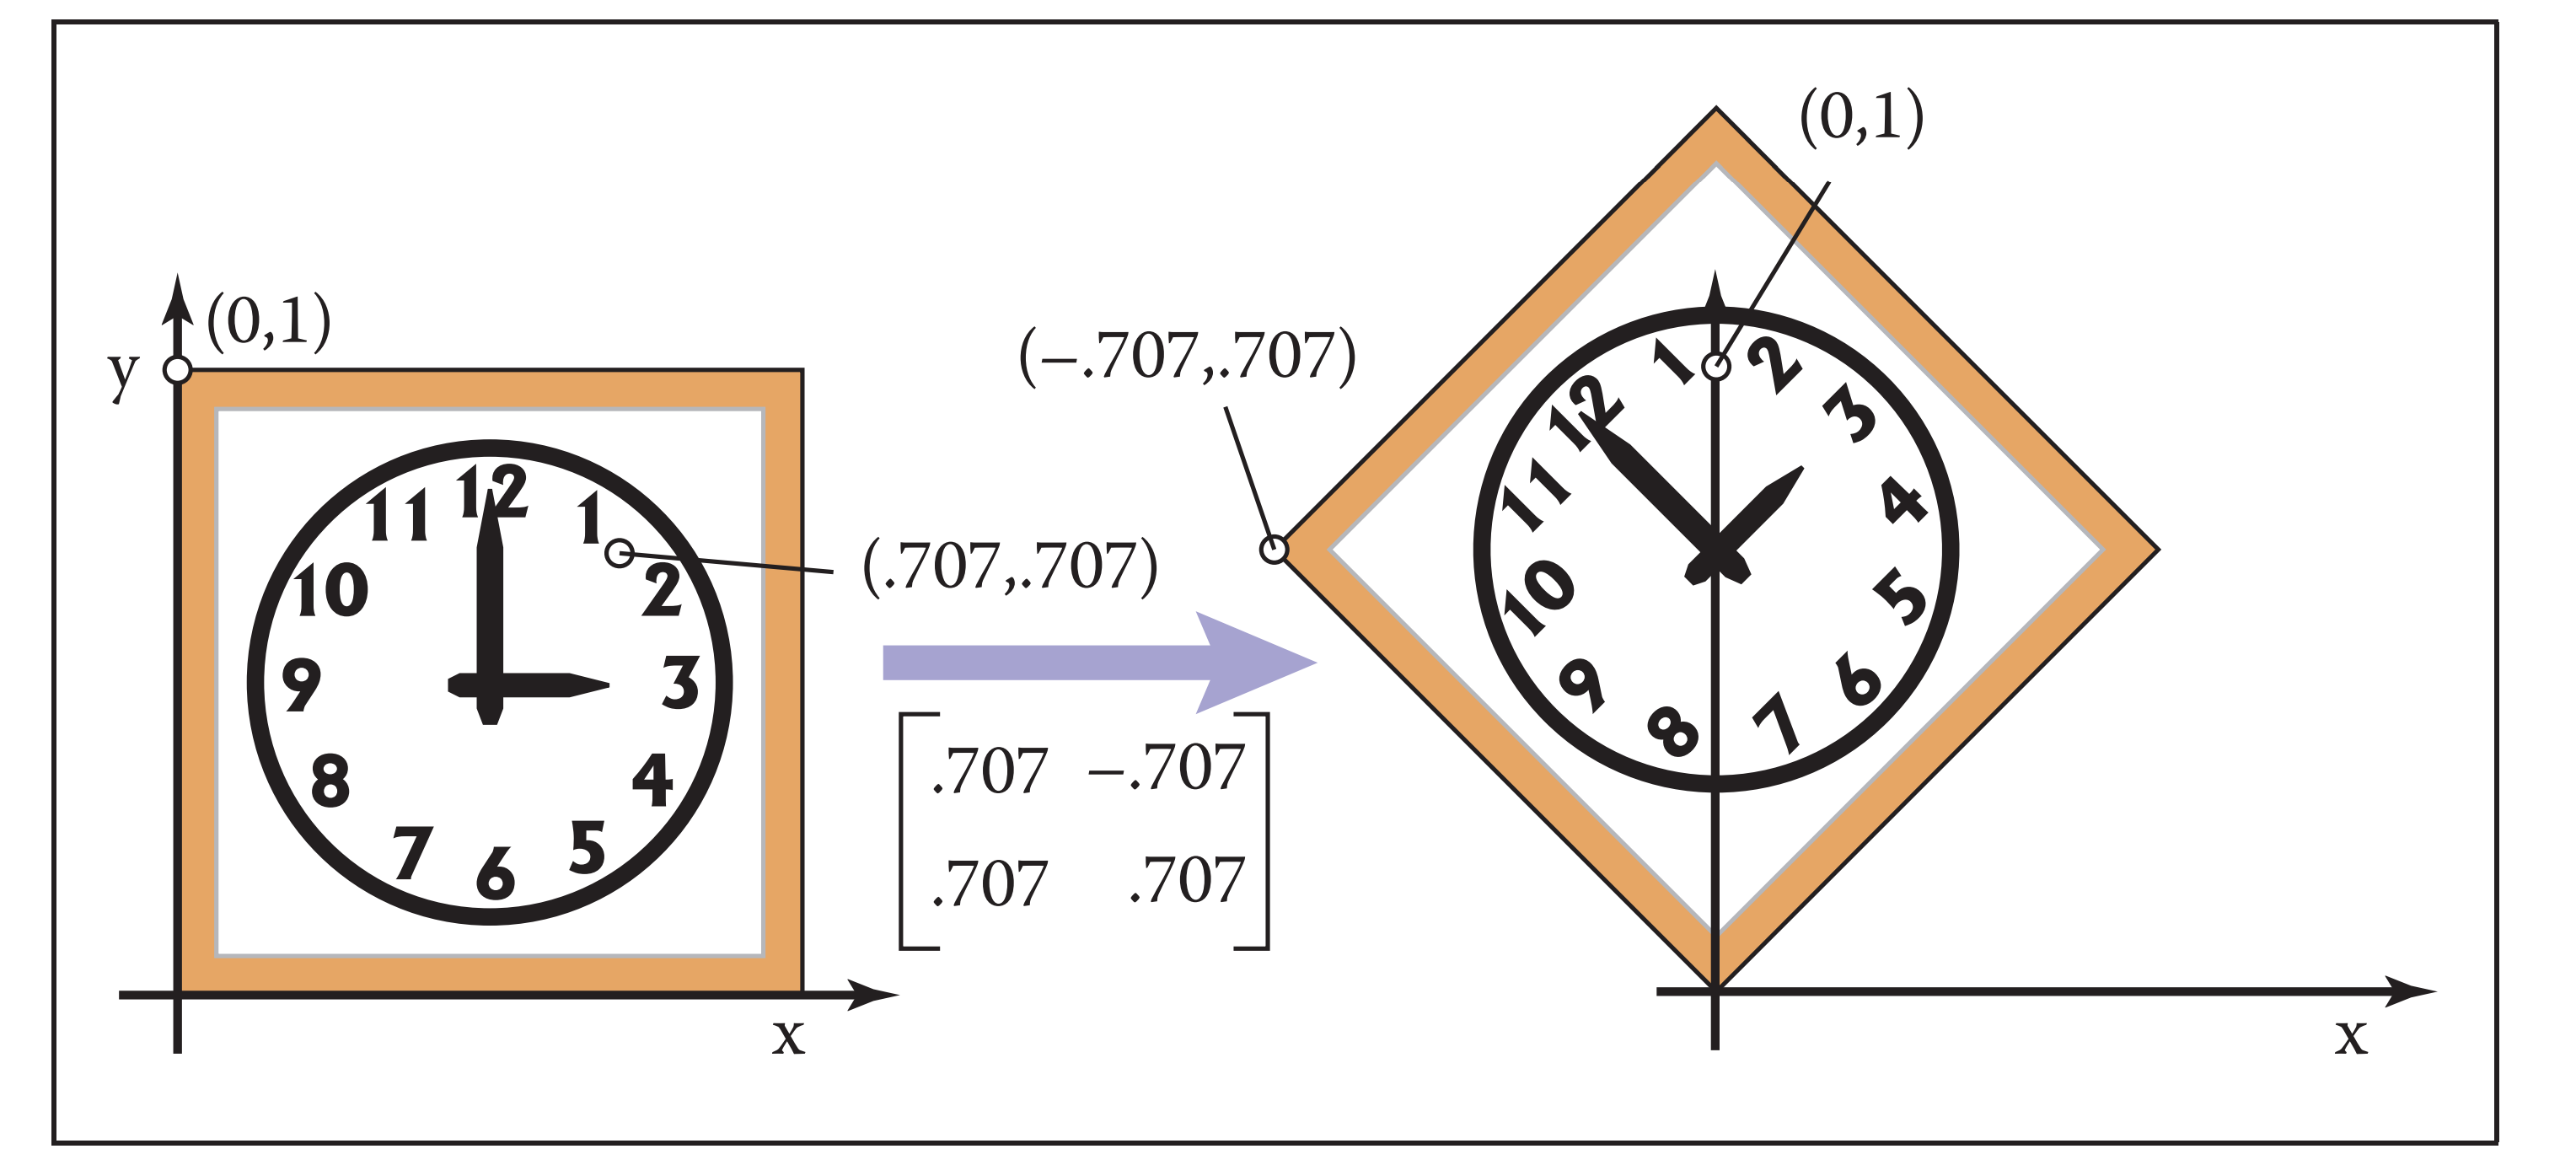
\includegraphics[scale=0.4]{Figure7.6.png}
		\caption{旋转$45^{\circ}$。注意到旋转是逆时针的,$cos(45^{\circ}) = sin(45^{\circ}) \approx .707 $}
		\label{fig:7.6}
	\end{figure}	
	
	顺时针方向旋转$\pi / 6$弧度($30^{\circ}$),在我们的框架中是旋转$-\pi / 6$弧度的旋转矩阵(如图\ref{fig:7.7}):
	
	\begin{equation}
		\left[\begin{array}{cr}
			\cos \frac{-\pi}{6} & -\sin \frac{-\pi}{6} \\
			\sin \frac{-\pi}{6} & \cos \frac{-\pi}{6}
		\end{array}\right]=\left[\begin{array}{rr}
			0.866 & 0.5 \\
			-0.5 & 0.866
		\end{array}\right] \text {. }
	\end{equation}
	
	\begin{figure}[htbp]
		\centering
		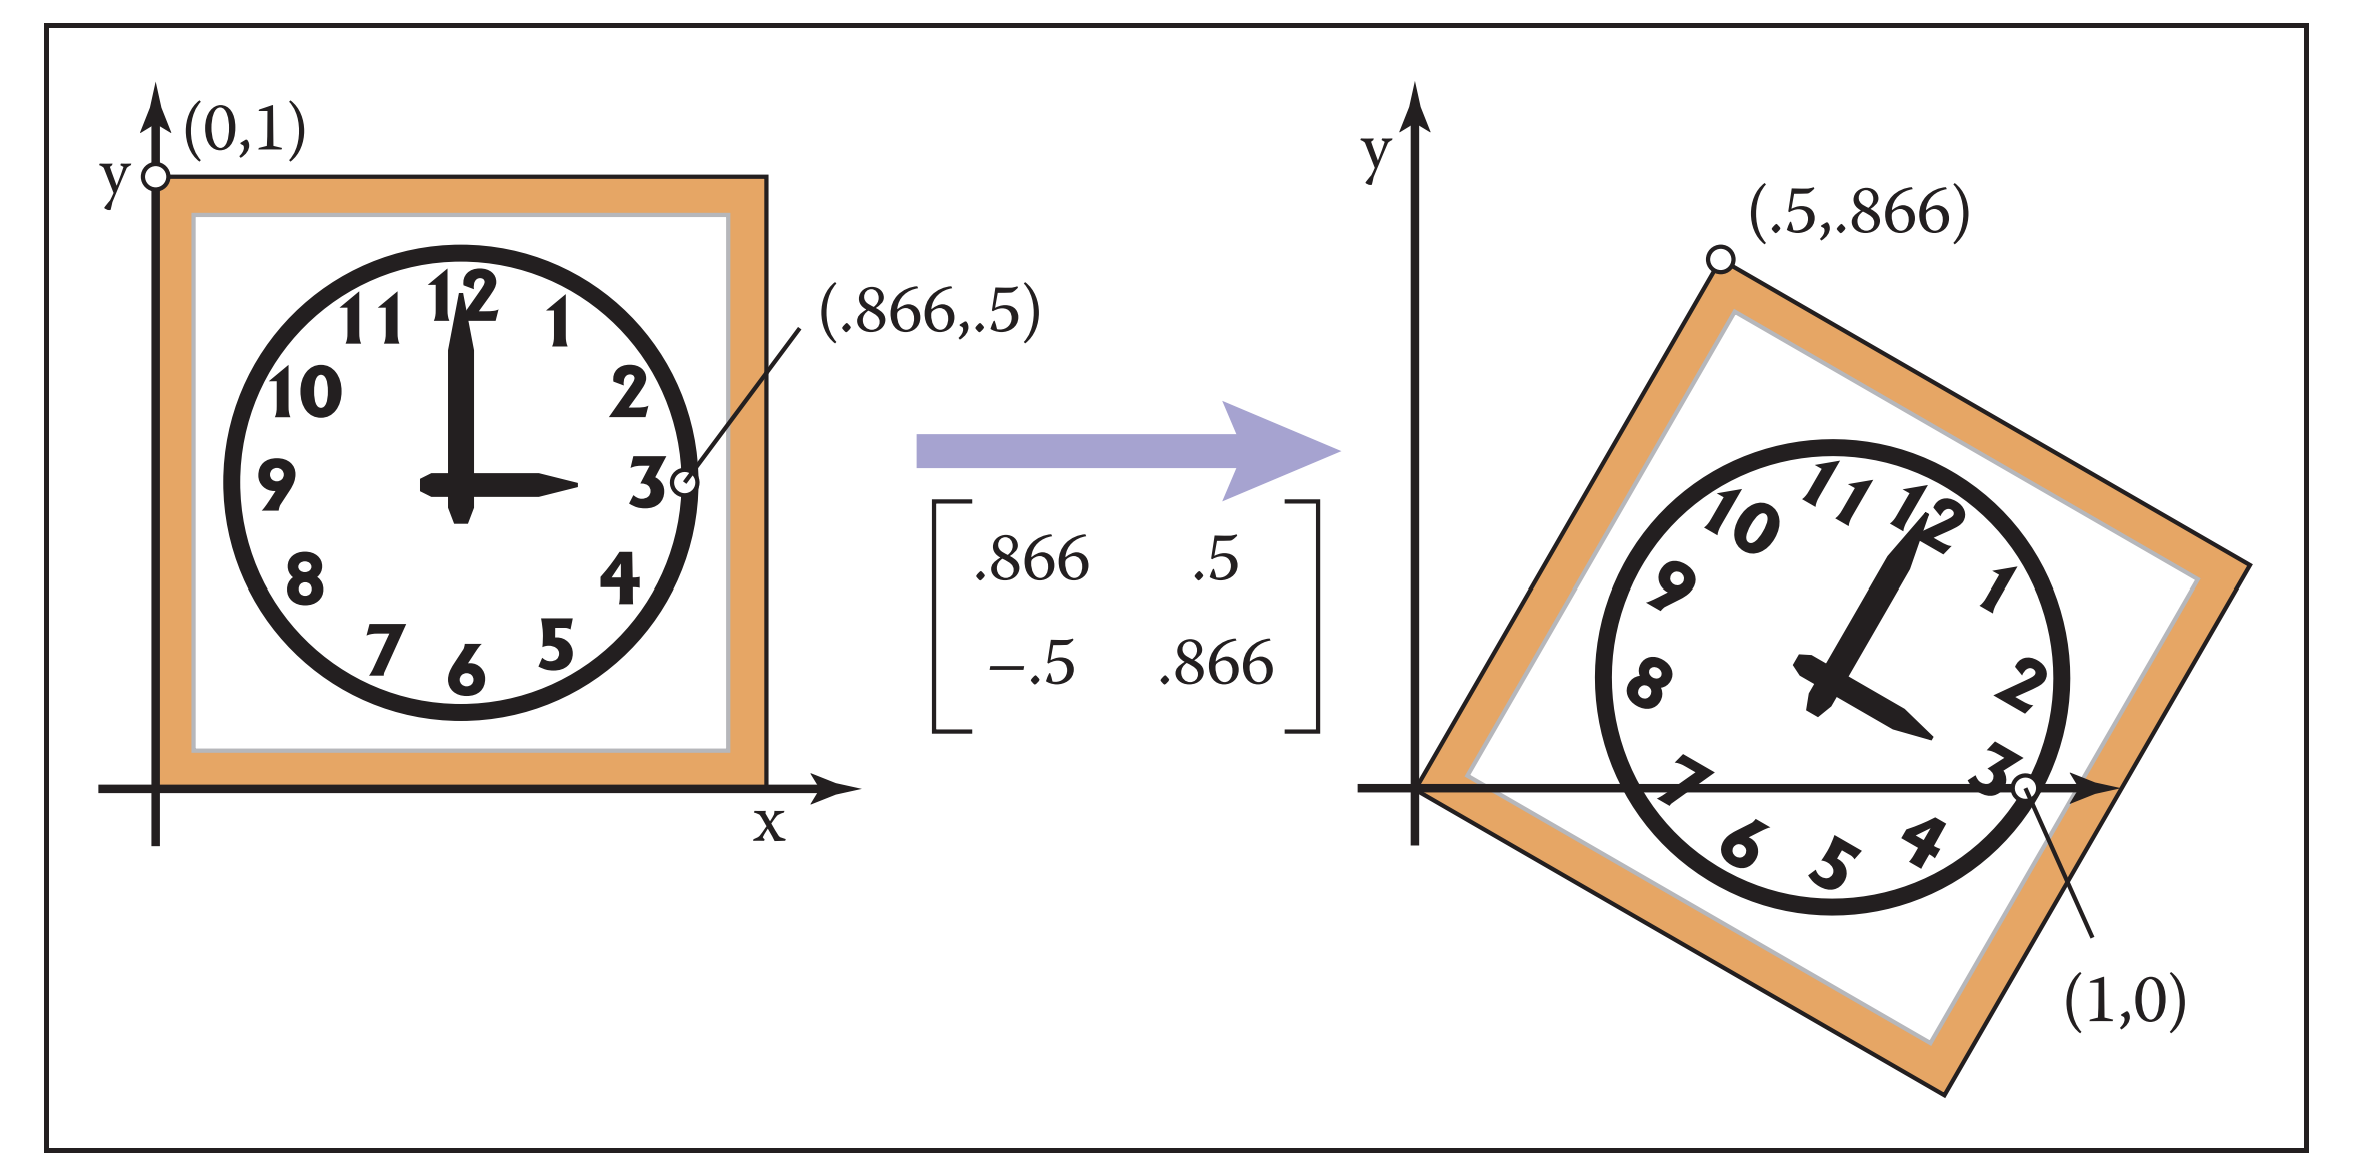
\includegraphics[scale=0.5]{Figure7.7.png}
		\caption{旋转$-30^{\circ}$。注意到旋转方向为顺时针,$cos(-30^{\circ}) \approx .866 $和$sin(-30^{\circ}) \approx -.5 $。}
		\label{fig:7.7}
	\end{figure}	
	
	
\end{example}

因为旋转矩阵每一行的范数是1$\left(\sin ^2 \phi+\cos ^2 \phi=1\right)$,并且行是正交的$(\cos \phi(-\sin \phi)+\sin \phi \cos \phi=0)$,我们看到旋转矩阵是正交矩阵(第\ref{5.2.4}节)。观察矩阵我们可以读出两对正交向量:两个列向量,(没看懂。。。)

\subsection{反射(Reflection)}

我们可以通过使用有一个负比例因子的比例矩阵来反射任一坐标轴上的向量(如图\ref{fig:7.8},图\ref{fig:7.9}):

\begin{equation}
	\text { reflect-y }=\left[\begin{array}{rr}
		-1 & 0 \\
		0 & 1
	\end{array}\right], \quad \text { reflect-x }=\left[\begin{array}{rr}
		1 & 0 \\
		0 & -1
	\end{array}\right]
\nonumber
\end{equation}

\begin{figure}[htbp]
	\centering
	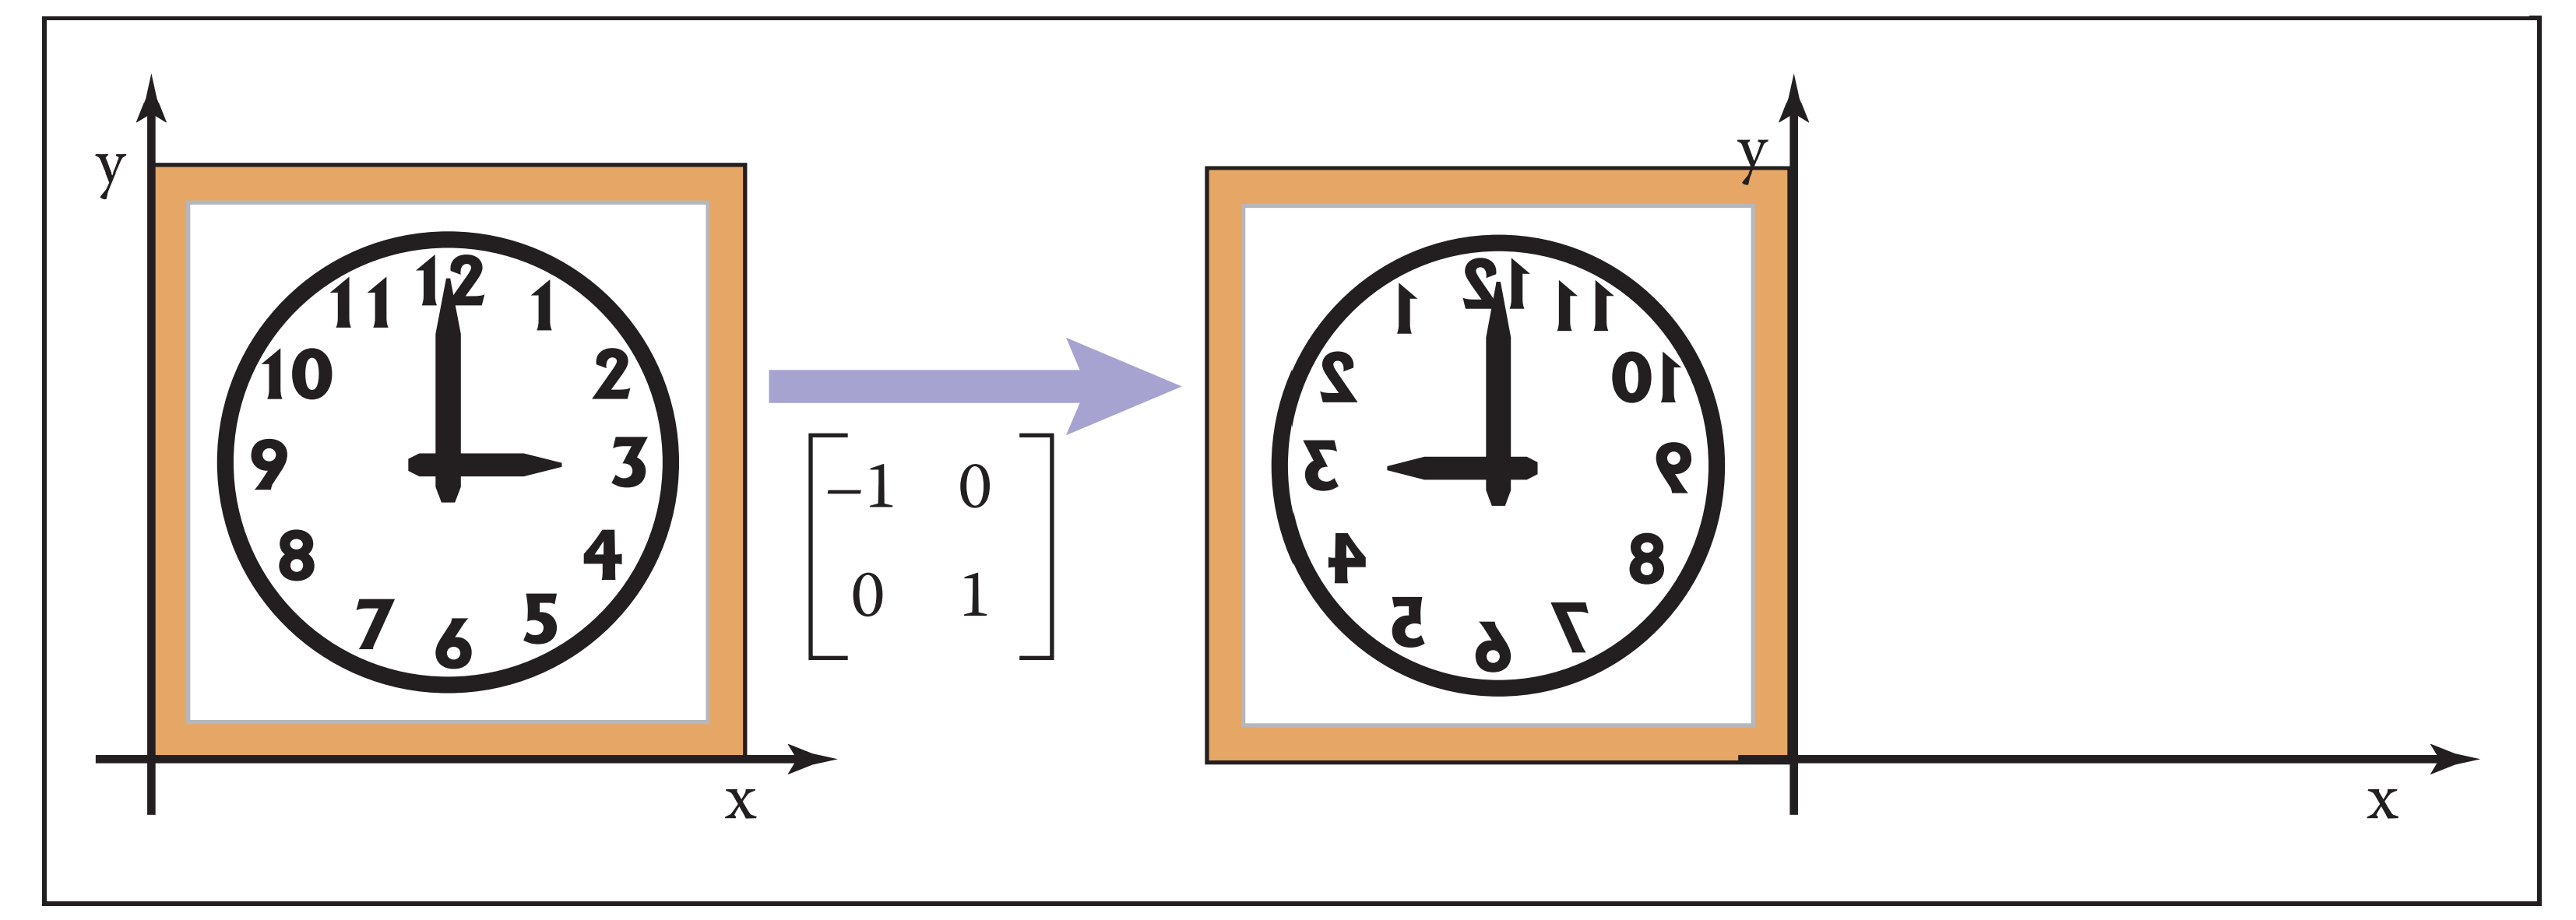
\includegraphics[scale=0.4]{Figure7.8.png}
	\caption{通过将所有x坐标乘以–1来实现关于y轴的反射。}
	\label{fig:7.8}
\end{figure}	

\begin{figure}[htbp]
	\centering
	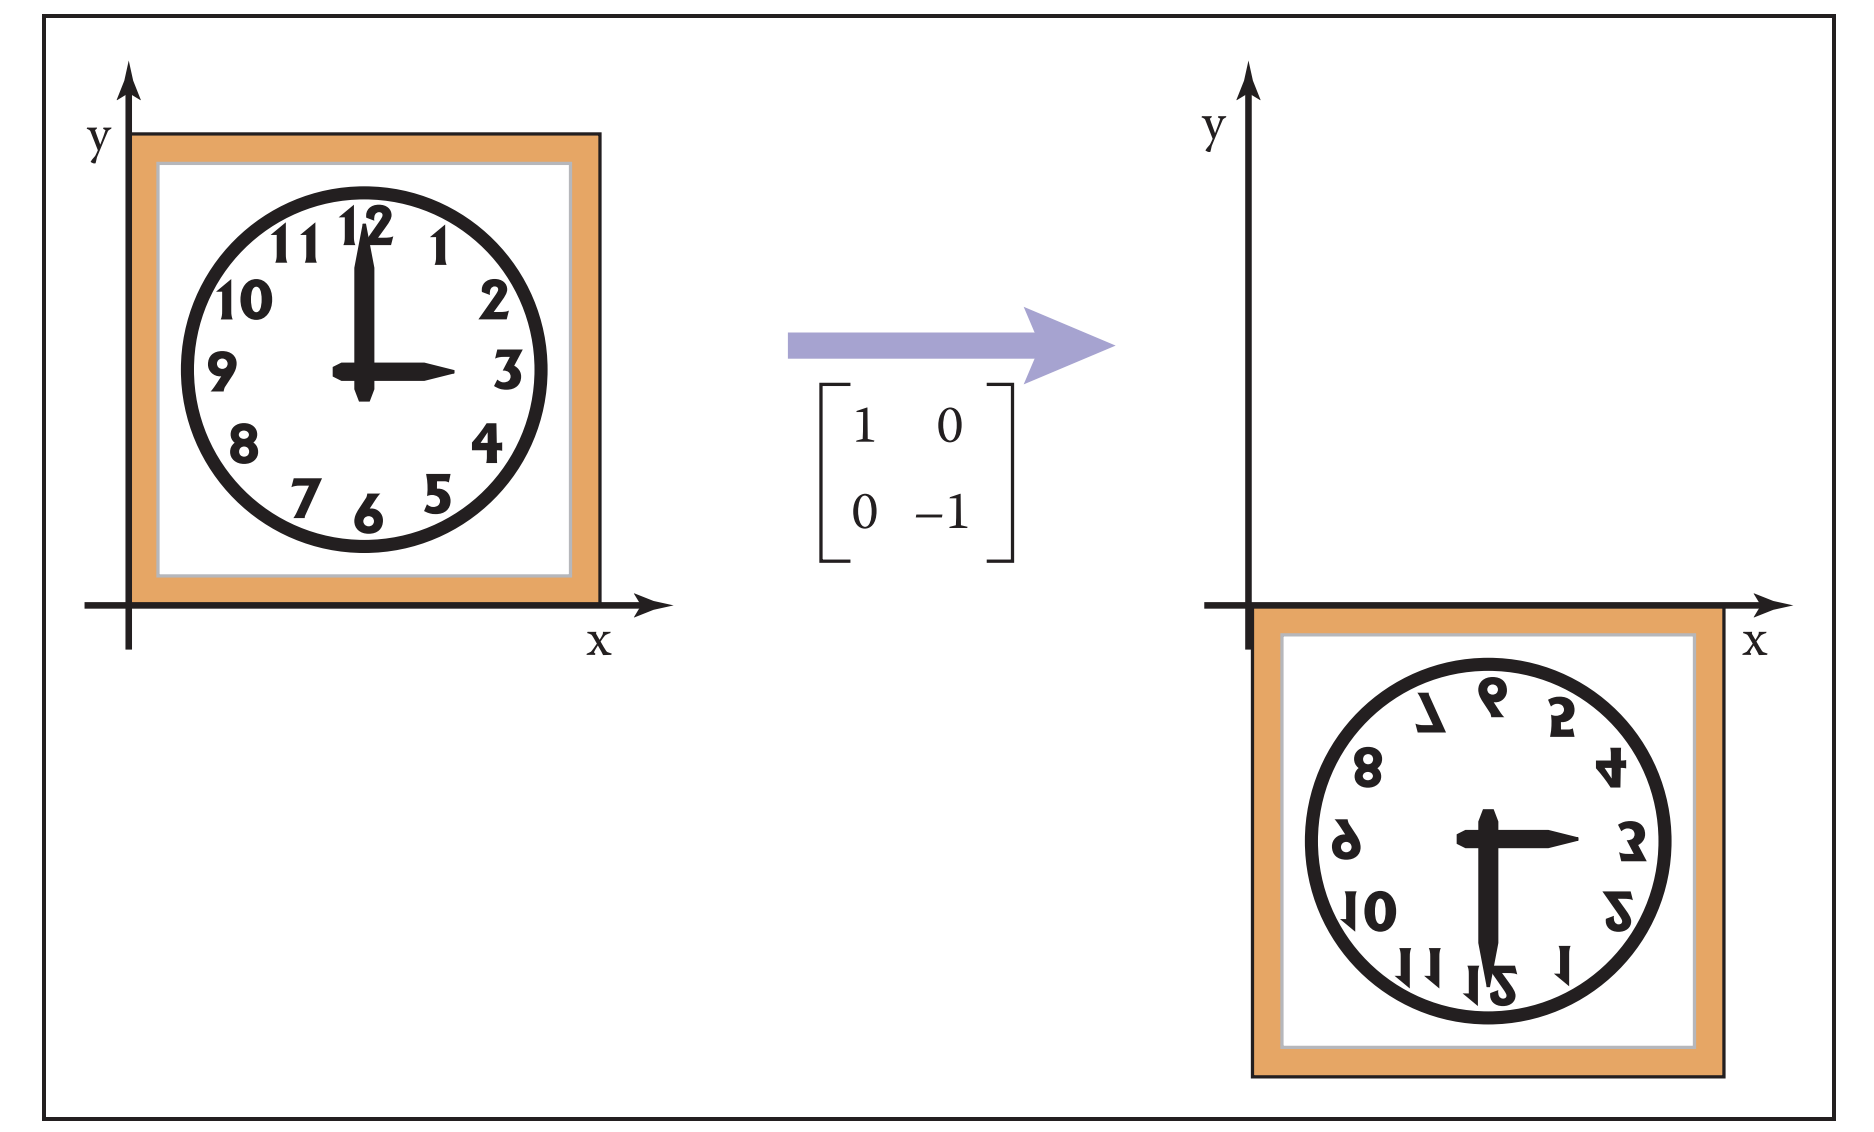
\includegraphics[scale=0.4]{Figure7.9.png}
	\caption{通过将所有y坐标乘以–1来实现关于x轴的反射。}
	\label{fig:7.9}
\end{figure}	

虽然人们可能会认为对角线的两个元素中都是−1的矩阵也是反射,但实际上它只是$\pi$弧度的旋转。

\subsection{变换的组成和分解(Composition and Decomposition of Transformations)}

图形程序通常对一个物体应用多个变换。例如,我们可能想先使用$\mathbf{S}$进行缩放,然后使用$\mathbf{R}$进行旋转。这将在二维向量$\mathbf{v}_{1}$上分两步完成:

\begin{equation}
	\text { first, } \mathbf{v}_2=\mathbf{S} \mathbf{v}_1, \text { then, } \mathbf{v}_3=\mathbf{R v}_2
	\nonumber
\end{equation}

另一种书写方式为:

\begin{equation}
	\mathbf{v}_3=\mathbf{R}\left(\mathbf{S v}_1\right)
	\nonumber
\end{equation}

因为矩阵乘法是满足结合律的,所以我们也可以写为:

\begin{equation}
	\mathbf{v}_3=(\mathbf{R S}) \mathbf{v}_1
	\nonumber
\end{equation}

换言之,我们可以使用相同大小的单个矩阵来表示由两个矩阵对向量变换的效果,我们可以将两个矩阵相乘来得到这个矩阵:$\mathbf{M}=\mathbf{R S}$(如图\ref{fig:7.10})。

请记住这些变换是从右侧进行变换的,这非常重要。所以矩阵$\mathbf{M}=\mathbf{R S}$先应用$\mathbf{S}$后应用$\mathbf{R}$。

\begin{figure}[htbp]
	\centering
	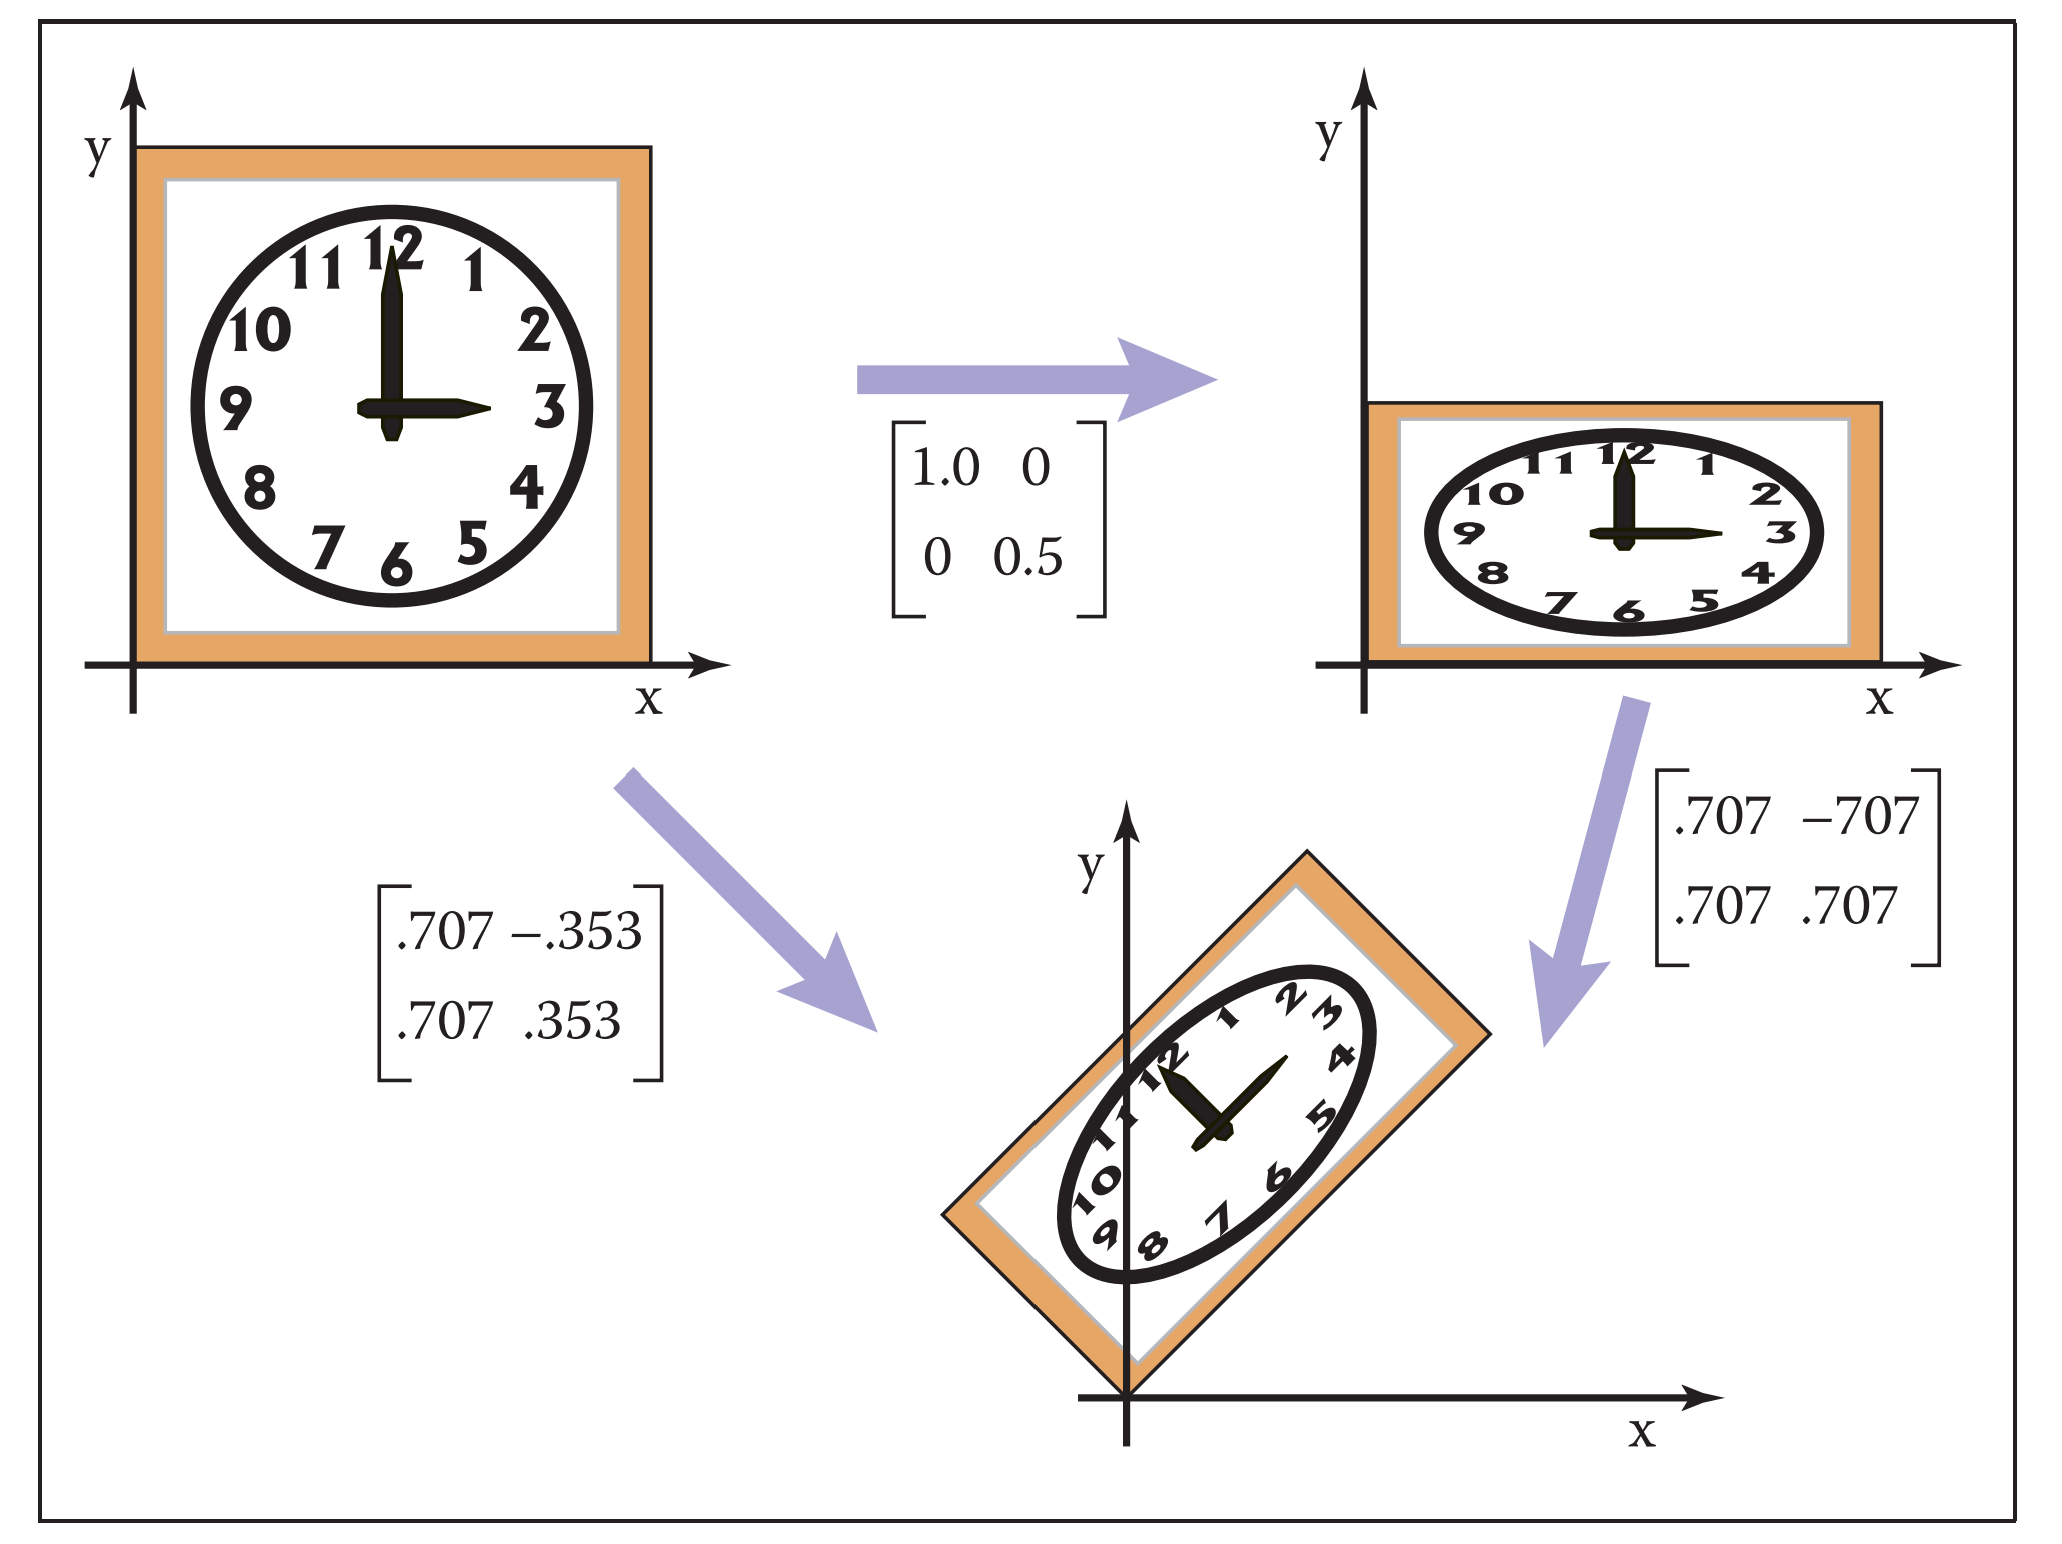
\includegraphics[scale=0.4]{Figure7.10.png}
	\caption{依次应用两个变换矩阵与应用一次这些矩阵的乘积是一样的。这是一个十分关键的概念,是大多数图形硬件和软件的基础。}
	\label{fig:7.10}
\end{figure}	

\begin{example}
	假设我们想在垂直方向上缩放一半,然后旋转$\pi/4$弧度($45^{\circ}$),其变换矩阵为:
	
	\begin{equation}
		\left[\begin{array}{cr}
			0.707 & -0.707 \\
			0.707 & 0.707
		\end{array}\right]\left[\begin{array}{cc}
			1 & 0 \\
			0 & 0.5
		\end{array}\right]=\left[\begin{array}{cc}
			0.707 & -0.353 \\
			0.707 & 0.353
		\end{array}\right]
	\nonumber
	\end{equation}

请务必记住矩阵乘法不是可交换的。所以变换的顺序很重要。对于这个例子,先进行旋转再进行缩放,是不同的变换矩阵(如图\ref{fig:7.11}):

\begin{equation}
	\left[\begin{array}{cc}
		1 & 0 \\
		0 & 0.5
	\end{array}\right]\left[\begin{array}{cr}
		0.707 & -0.707 \\
		0.707 & 0.707
	\end{array}\right]=\left[\begin{array}{rr}
		0.707 & -0.707 \\
		0.353 & 0.353
	\end{array}\right]
\nonumber
\end{equation}

\begin{figure}[htbp]
	\centering
	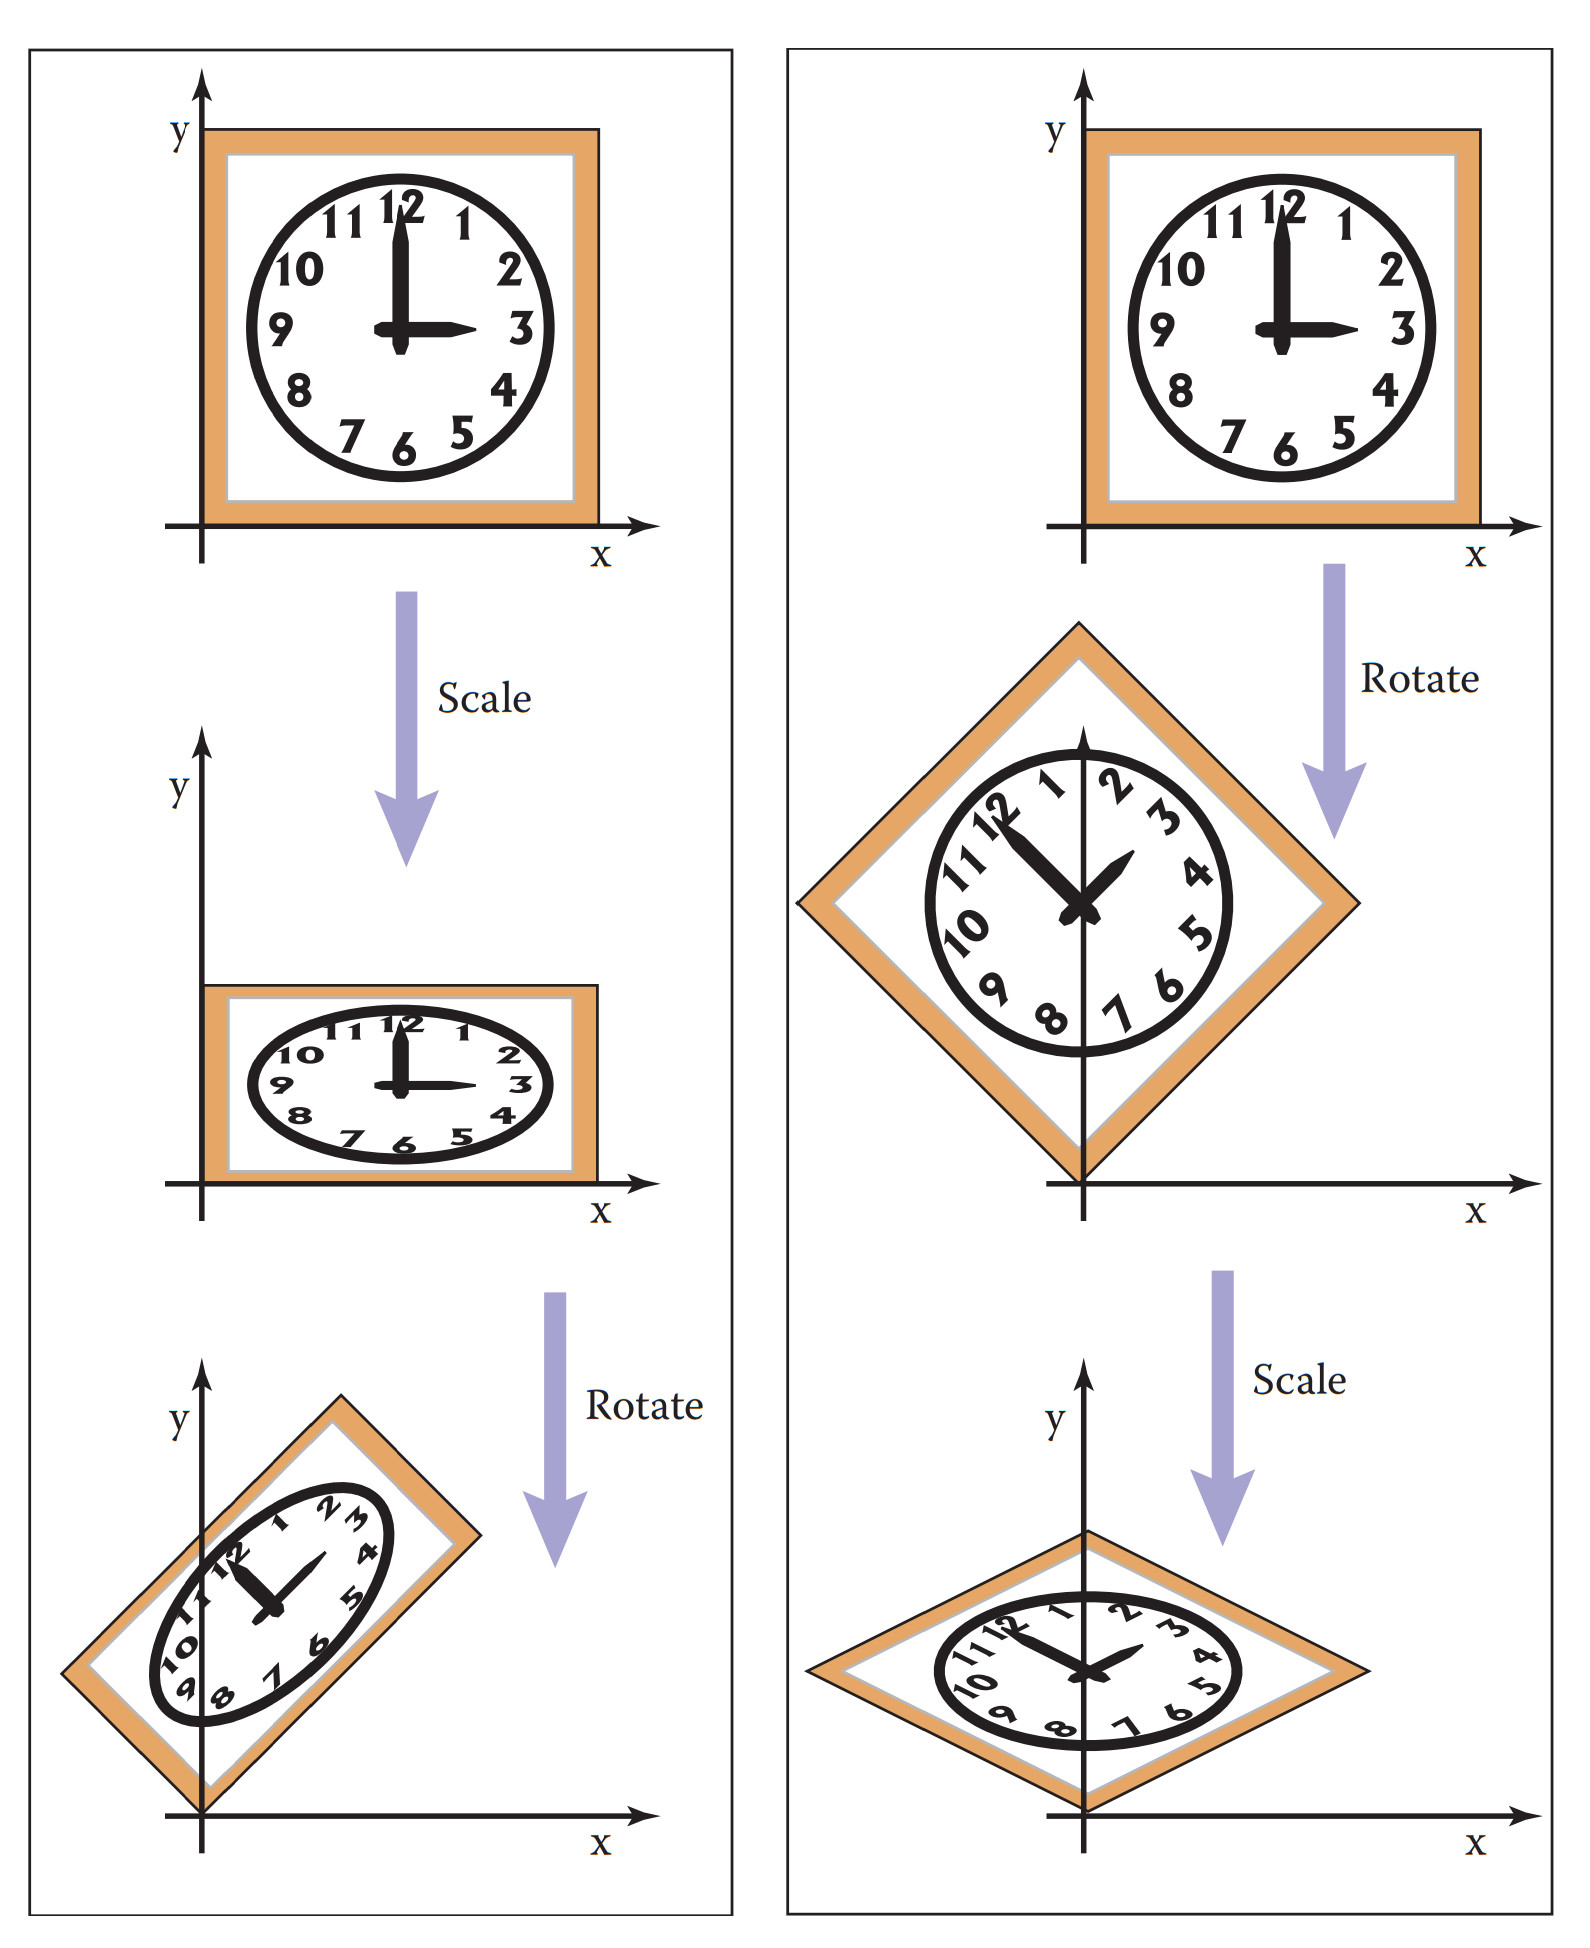
\includegraphics[scale=0.55]{Figure7.11.png}
	\caption{应用两种变换的顺序通常很重要。对于这个例子,我们在y轴上做了二分之一的缩放,然后旋转了$45^{\circ}$。将这两个变换的顺序颠倒一下,会产生不同的结果。}
	\label{fig:7.11}
\end{figure}	

\end{example}

\begin{example}
	使用我们提出的缩放矩阵,非均匀缩放只能沿坐标轴进行。如果我们想拉伸沿着时钟的一条对角线拉伸时钟50\%,使8:00到1:00移动到西北方向,2:00到7:00移动到东南方向,我们可以使用一个结合了轴对齐缩放矩阵的旋转矩阵来达到这个目的。其想法是使用旋转将缩放轴与坐标轴对齐,然后沿该轴缩放,然后旋转回来。在我们的示例中,缩放轴是正方形的“反斜杠”对角线,我们可以使其与$x$轴平行,旋转$+45^{\circ}$。将这些操作放在一起,完整的变换矩阵是:
	
	\begin{equation}
		\operatorname{rotate}\left(-45^{\circ}\right) \operatorname{scale}(1.5,1) \operatorname{rotate}\left(45^{\circ}\right)
		\nonumber
	\end{equation}
	
	在数学符号中,这可以写成$\mathbf{R}\mathbf{S}\mathbf{R}^{\mathbf{T}}$。将三个矩阵相乘的结果是:
	
	\begin{equation}
		\left[\begin{array}{cc}
			1.25 & -0.25 \\
			-0.25 & 1.25
		\end{array}\right]
	\nonumber
	\end{equation}
	
	从旋转和缩放变换中建立起的变换实际上对任何线性变换都是有效的,这诱导我们对这些变换进行强烈的思考,在下一节将进行探讨。
	
\end{example}

\subsection{变换的分解(Decomposition of Transformations)}

有时有必要 "撤销 "一个变换的组合,把一个变换拆成更简单的部分。例如,相对于单独的旋转和缩放,以变换矩阵的形式呈现给用户进行操作通常是有用的,但是一个变换可能被简单地表示为一个矩阵,旋转和缩放已经混合在一起。如果可以通过计算将矩阵分解成所需的部分,调整这些部分,并通过将这些部分再次相乘来重新组装矩阵,就可以实现这种操作。

事实证明,这种分解或矩阵分解是可能的,不管矩阵中的内容是什么。这提供了一种很有效的方式来思考变换以及它们对变换的几何体所做的操作。

\subsubsection*{\textcolor{structure3}{对称特征值分解(Symmetric Eigenvalue Decomposition)}}

让我们从对称阵开始。还记得第\ref{6.4}小节说过,对称阵总是可以通过特征值分解以下矩阵相乘的形式:

\begin{equation}
    \mathbf{A} = \mathbf{R}\mathbf{S}\mathbf{R}^{\mathbf{T}}
    \nonumber
\end{equation}

其中,$\mathbf{R}$是正交阵,$\mathbf{S}$是对角阵;我们称$\mathbf{R}$的列(特征向量)为$\mathbf{v}_{1}$和$\mathbf{v}_{2}$,称$\mathbf{S}$的对象项为$\lambda_{1}$和$\lambda_{2}$。

在几何术语中,我们现在可以认出$\mathbf{R}$是旋转变换,$\mathbf{S}$是缩放变换,因此这只是一个多步骤的几何变换(图\ref{fig:7.12}):

\begin{enumerate}
	\item 将$\mathbf{v}_{1}$和$\mathbf{v}_{2}$旋转到$x$轴和$y$轴上(旋转矩阵$\mathbf{R}^{T}$)。
	
	\item 通过$lambda_{1}$和$\lambda_{2}$缩放$x$和$y$(缩放矩阵$\mathbf{S}$)。
	
	\item 将$x$轴和$y$轴旋转回到$\mathbf{v}_{1}$和$\mathbf{v}_{2}$上(旋转矩阵$\mathbf{R}$)。
\end{enumerate}

\begin{figure}[htbp]
	\centering
	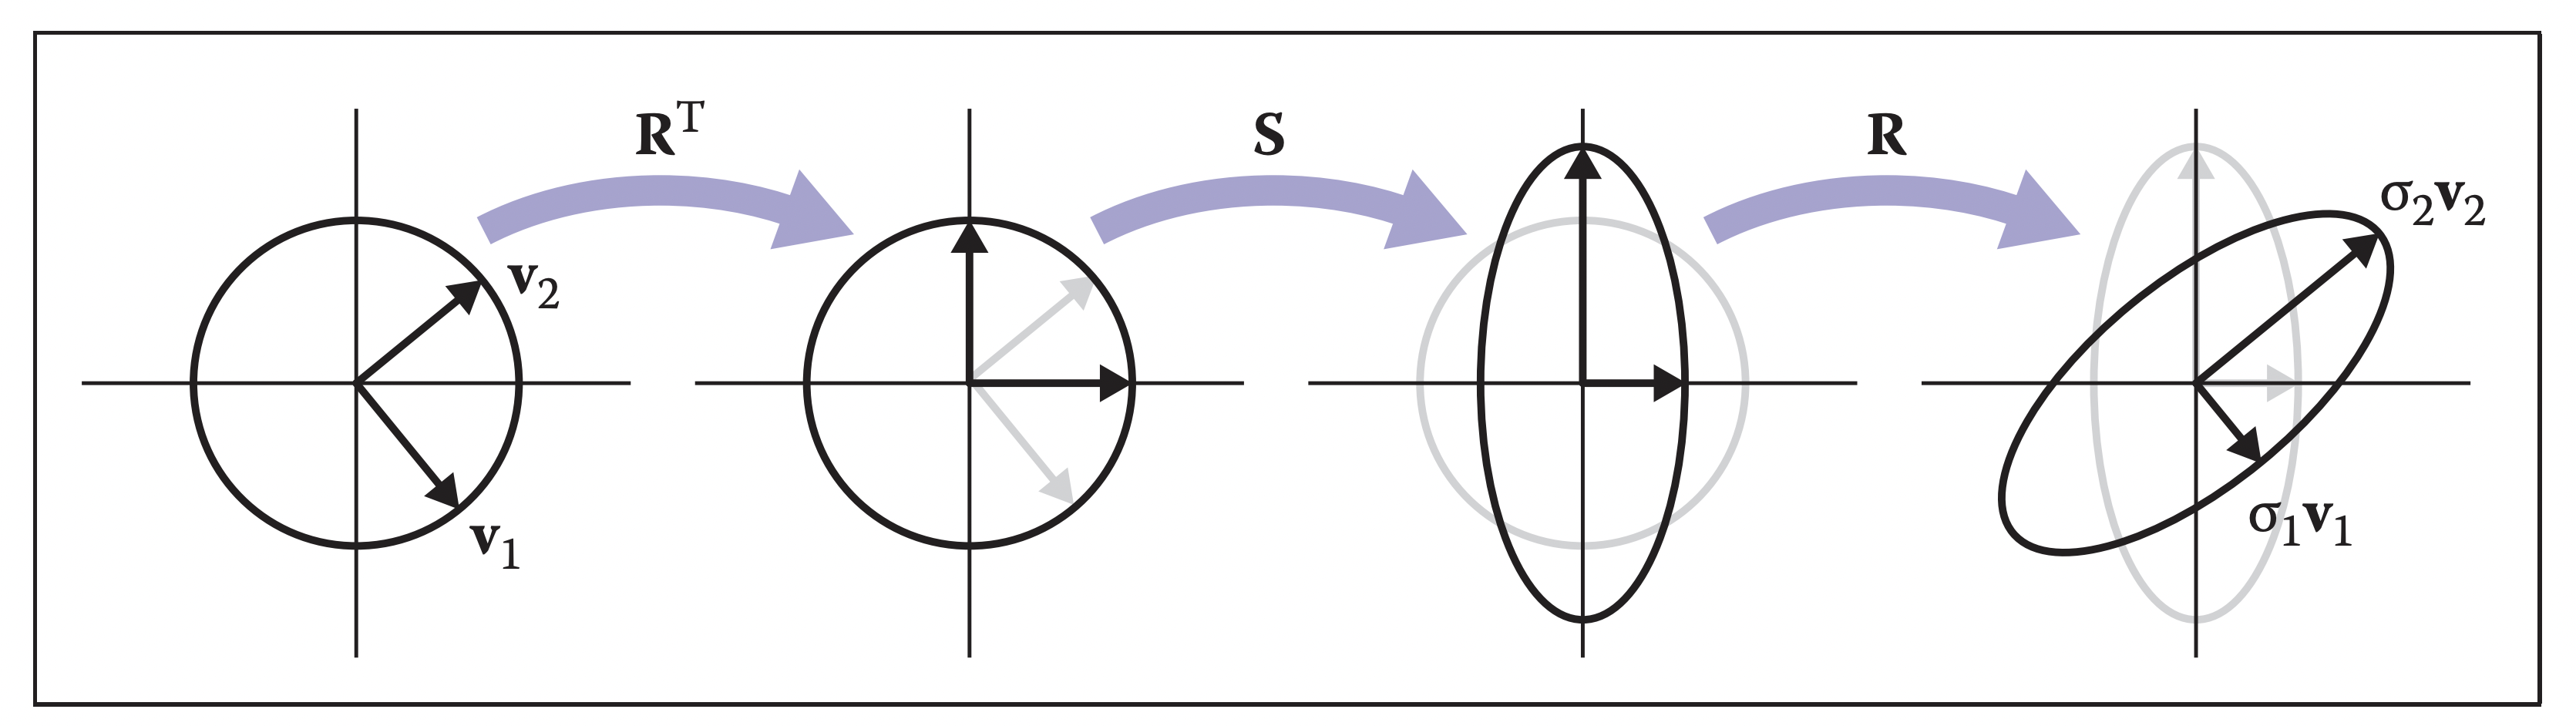
\includegraphics[scale=0.27]{Figure7.12.png}
	\caption{当一个单位圆被一个任意的对称矩阵也就是非轴对齐、非均匀的矩阵$\mathbf{A}$进行转换时会发生什么。作为矩阵$\mathbf{A}$特征向量的两个垂直向量$\mathbf{v}_{1}$和$\mathbf{v}_{2}$保持了它们本来的方向,但是被缩放了。对于初等变换,这可以等价于首先将特征向量旋转到正则基,进行轴对齐的缩放,然后将正则基旋转回特征向量。}
	\label{fig:7.12}
\end{figure}	

把这三个变换的效果放在一起看,我们可以发现他们有将物体沿着一对轴进行非均匀缩放的效果。和轴对齐的缩放一样,两个轴是垂直的,但它们不是坐标轴,而是$\mathbf{A}$的特征向量\footnote{如果你喜欢计算维度:一个对称的$2 \times 2$的矩阵有3个自由度,而特征值分解将它们写为一个旋转角度和两个比例因子。}。这告诉我们关于对称矩阵的含义:对称矩阵只是一种缩放操作——尽管可能是不均匀的和非轴对齐的。

\begin{example}
回忆第\ref{5.4}小节的例子:

\begin{equation}
	\begin{aligned}
		{\left[\begin{array}{ll}
				2 & 1 \\
				1 & 1
			\end{array}\right] } & =\mathbf{R}\left[\begin{array}{cc}
			\lambda_1 & 0 \\
			0 & \lambda_2
		\end{array}\right] \mathbf{R}^{\mathrm{T}} \\
		& =\left[\begin{array}{cc}
			0.8507 & -0.5257 \\
			0.5257 & 0.8507
		\end{array}\right]\left[\begin{array}{cc}
			2.618 & 0 \\
			0 & 0.382
		\end{array}\right]\left[\begin{array}{cc}
			0.8507 & 0.5257 \\
			-0.5257 & 0.8507
		\end{array}\right] \\
		& =\operatorname{rotate}\left(31.7^{\circ}\right) \operatorname{scale}(2.618,0.382) \operatorname{rotate}\left(-31.7^{\circ}\right) .
	\end{aligned}
\nonumber
\end{equation}

The matrix above, then, according to its eigenvalue decomposition, scales in a
direction $31.7^{\circ}$ counterclockwise from three o’clock (the x-axis). This is a touch
before 2 p.m. on the clockface as is confirmed by Figure \ref{fig:7.13}.(没看懂这句话。。。感觉应该说的是先进行了旋转,然后拉伸,再转回去。)

\begin{figure}[htbp]
	\centering
	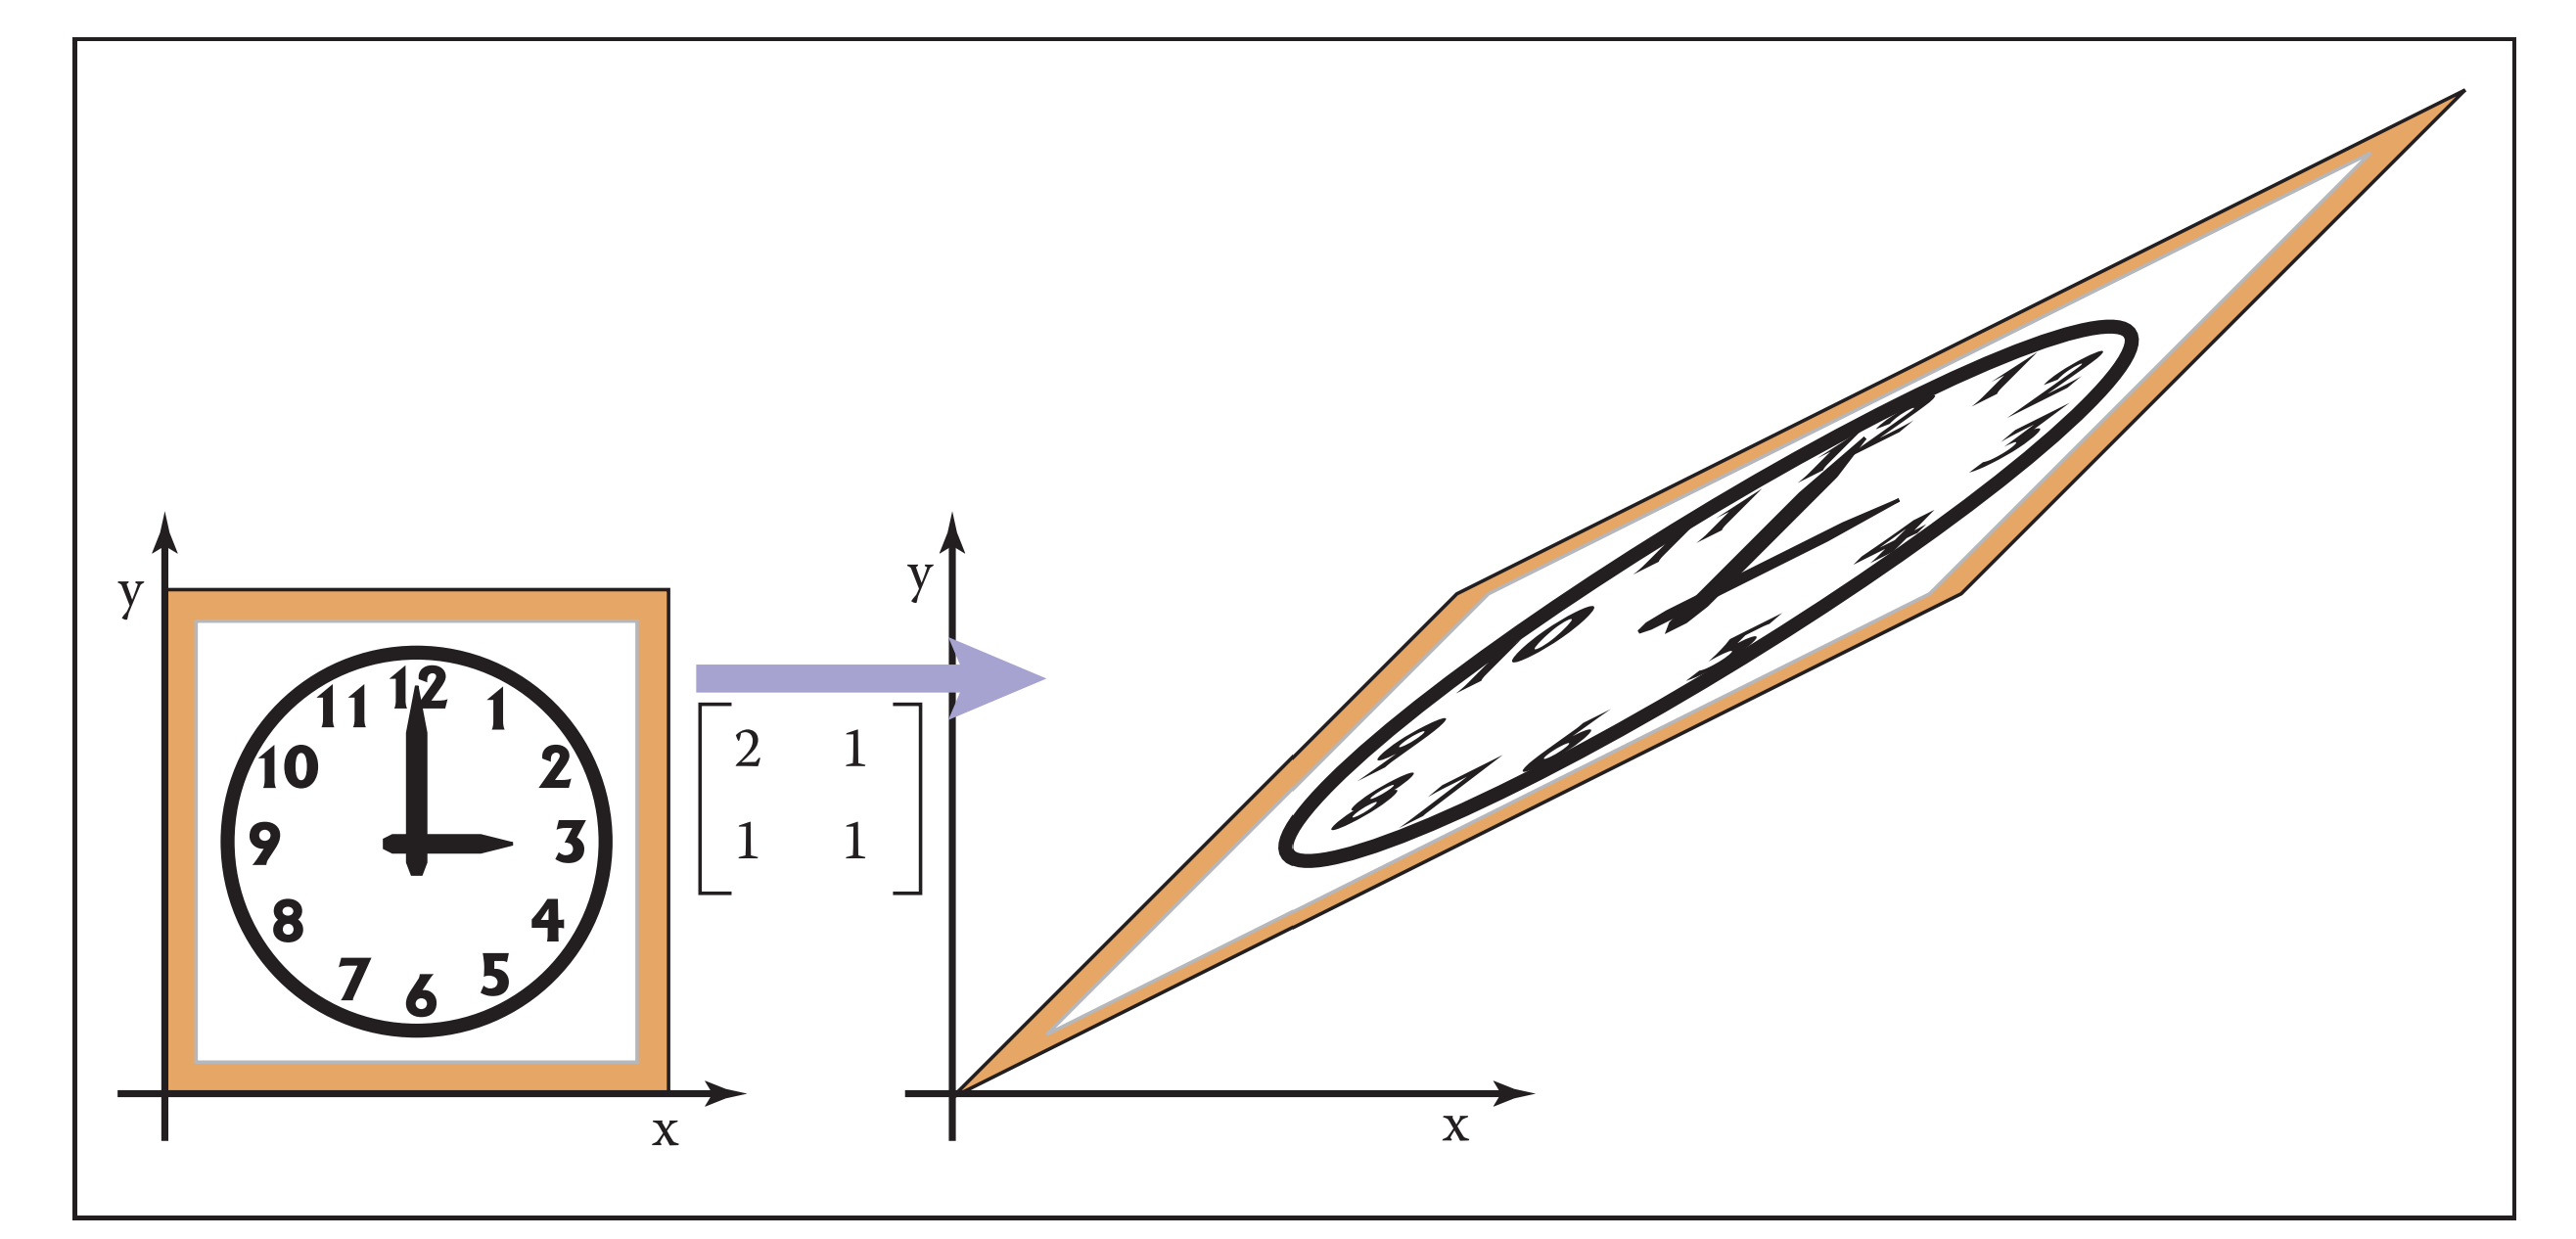
\includegraphics[scale=0.4]{Figure7.13.png}
	\caption{对称矩阵总是沿着某个轴进行缩放。在这种情况下,它沿着$\phi = 31.7^{\circ}$方向,这意味着这个矩阵的特征向量在这个方向上。}
	\label{fig:7.13}
\end{figure}	

我们也可以将对角线化的过程倒过来;以$(\lambda_{1},\lambda_{2})$为比例,第一个比例方向为从X轴顺时针方向的角度$\phi$,我们有:

\begin{equation}
	\begin{aligned}
		{\left[\begin{array}{rr}
				\cos \phi & \sin \phi \\
				-\sin \phi & \cos \phi
			\end{array}\right]\left[\begin{array}{cc}
				\lambda_1 & 0 \\
				0 & \lambda_2
			\end{array}\right]\left[\begin{array}{rr}
				\cos \phi & -\sin \phi \\
				\sin \phi & \cos \phi
			\end{array}\right]=} & \\
		& {\left[\begin{array}{ll}
				\lambda_1 \cos ^2 \phi+\lambda_2 \sin ^2 \phi & \left(\lambda_2-\lambda_1\right) \cos \phi \sin \phi \\
				\left(\lambda_2-\lambda_1\right) \cos \phi \sin \phi & \lambda_2 \cos ^2 \phi+\lambda_1 \sin ^2 \phi
			\end{array}\right] . }
	\end{aligned}
\nonumber
\end{equation}

我们应该感到欣慰的是,这是一个如假包换的对称矩阵,因为我们从对称的特征值分解中构建了它。

\end{example}


\subsubsection*{\textcolor{structure3}{奇异值分解(Singular Value Decomposition)}}

非对称矩阵也可以进行非常相似的分解:奇异值分解(SVD),在第5.4.1节中有讨论。不同的是,对角矩阵两边的矩阵不再相同:

\begin{equation}
	\mathbf{A}=\mathbf{U S V}^{\mathrm{T}}
	\nonumber
\end{equation}

取代旋转矩阵$\mathbf{R}$的两个正交矩阵被称为$\mathbf{U}$和$\mathbf{V}$,它们的列向量分别被称为$\mathbf{u}_{i}$(左奇异向量)和$\mathbf{v}_{i}$(右奇异向量)。

在这种情况下,S的对角项被称为奇异值,而不是特征值。几何解释与对称特征值分解非常相似(图\ref{fig:7.14})

\begin{figure}[htbp]
	\centering
	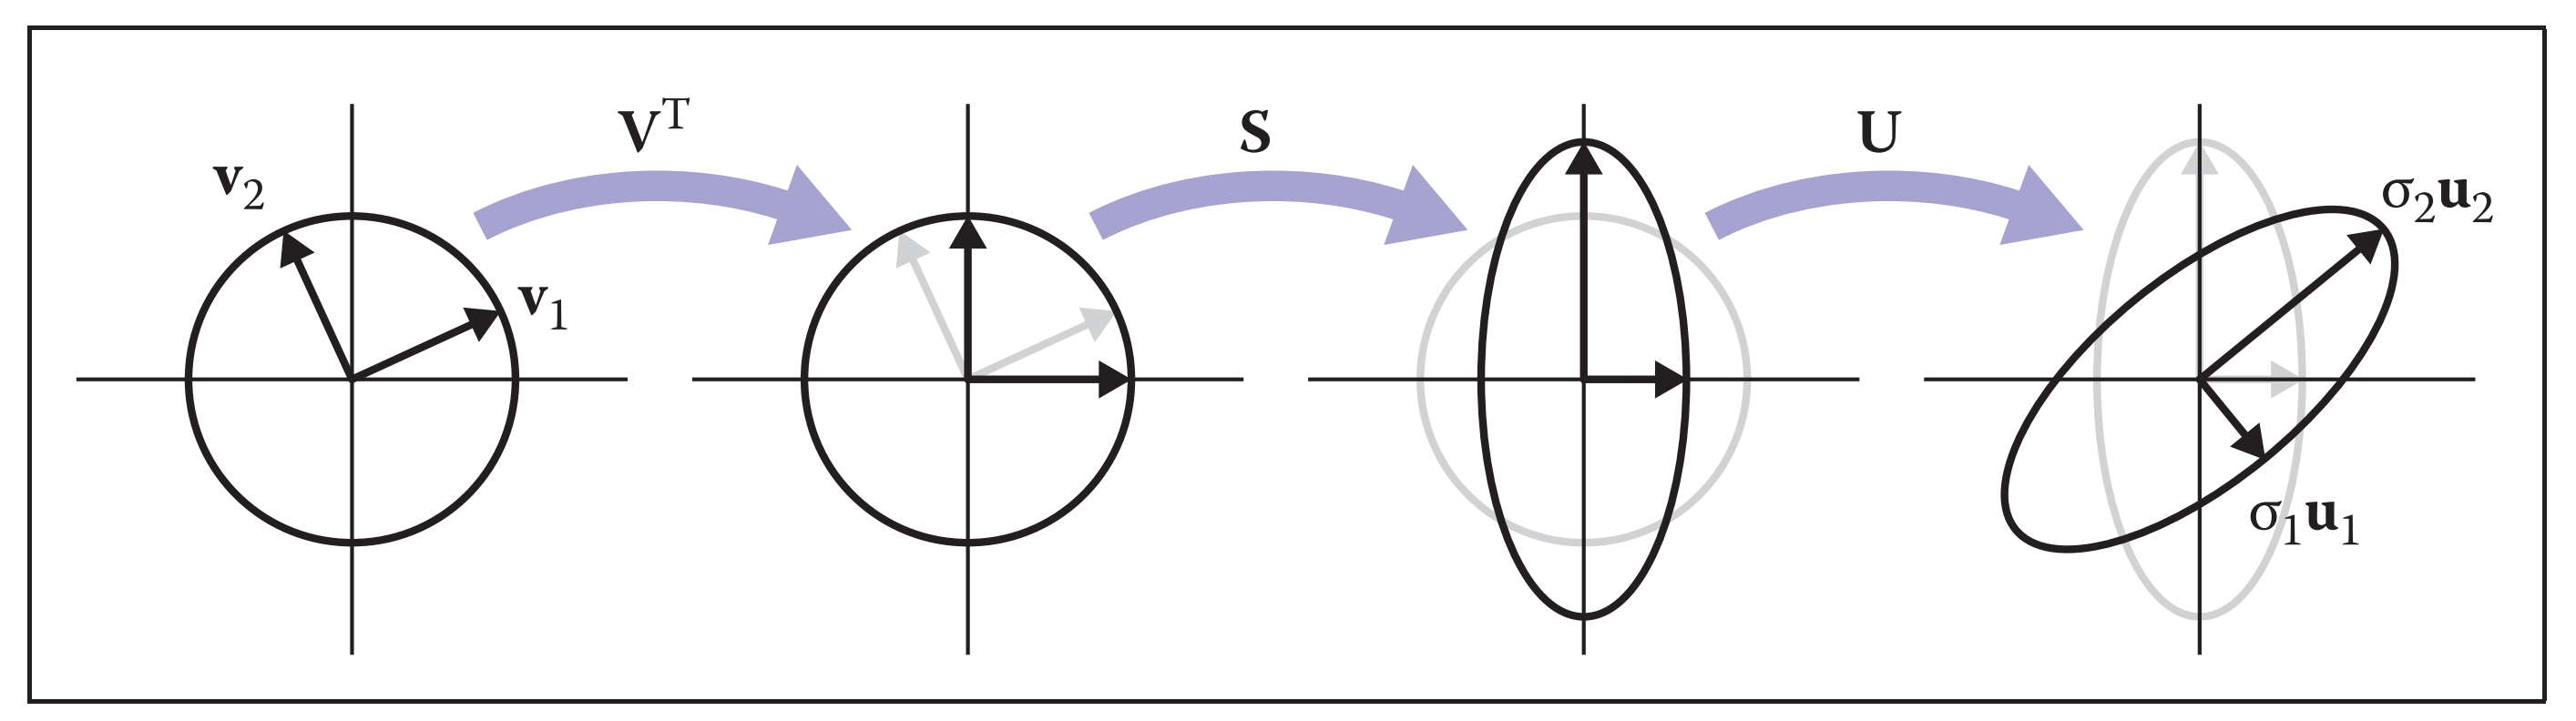
\includegraphics[scale=0.45]{Figure7.14.png}
	\caption{当一个单位圆被一个任意的对称矩阵也就是非轴对齐、非均匀的矩阵$\mathbf{A}$进行转换时会发生什么。作为矩阵$\mathbf{A}$特征向量的两个垂直向量$\mathbf{v}_{1}$和$\mathbf{v}_{2}$保持了它们本来的方向,但是被缩放了。对于初等变换,这可以等价于首先将右奇异向量旋转到正则基,进行轴对齐的缩放,然后将正则基旋转回左奇异向量。}
	\label{fig:7.14}
\end{figure}	

\begin{enumerate}
	\item 将$\mathbf{v}_{1}$和$\mathbf{v}_{2}$旋转到$x$轴和$y$轴上(旋转矩阵$\mathbf{V}^{T}$)。
	
	\item 通过$\sigma_{1}$和$\sigma_{2}$缩放$x$和$y$(缩放矩阵$\mathbf{S}$)。
	
	\item 将$x$轴和$y$轴旋转回到$\mathbf{v}_{1}$和$\mathbf{v}_{2}$上(旋转矩阵$\mathbf{U}$)。
\end{enumerate}

主要的区别就在旋转矩阵$\mathbf{R}$和两个不同的正交矩阵$\mathbf{V}$和$\mathbf{U}$。这种差异导致了另一个不太重要的差异。因为$\mathbf{SVD}$的两边有不同的奇异向量,所以不需要负的奇异值:我们总是可以改变一个奇异值的正负,然后翻转与其对应奇异向量的方向,最后得到相同的变换。如此,$\mathbf{SVD}$总是产生一个所有正项的对角矩阵,但是矩阵$\mathbf{U}$和$\mathbf{V}$并不保证是旋转--它们也可能包括反射。在几何应用例如图形学中,这是一个不便之处,但也只是一个小问题:通过检查行列式,很容易区分旋转和反射,旋转的行列式是$+1$,反射的行列式是$\textnormal{-}1 $。如果需要旋转,可以翻转其中一个奇异值的正负,从而产生一个旋转-缩放-旋转的序列,其中反射与缩放一起滚动,而不是与其中一个旋转一起(没看懂,原文: where the reflection is
rolled in with the scale, rather than with one of the rotations.)。

\begin{example}在第\ref{5.4.1}小节使用的例子实际上是剪切矩阵(图\ref{fig:7.12}):
	\begin{equation}
		\begin{aligned}
			{\left[\begin{array}{ll}
					1 & 1 \\
					0 & 1
				\end{array}\right] } & =\mathbf{R}_2\left[\begin{array}{cc}
				\sigma_1 & 0 \\
				0 & \sigma_2
			\end{array}\right] \mathbf{R}_1 \\
			& =\left[\begin{array}{cc}
				0.8507 & -0.5257 \\
				0.5257 & 0.8507
			\end{array}\right]\left[\begin{array}{cc}
				1.618 & 0 \\
				0 & 0.618
			\end{array}\right]\left[\begin{array}{rr}
				0.5257 & 0.8507 \\
				-0.8507 & 0.5257
			\end{array}\right] \\
			& =\operatorname{rotate}\left(31.7^{\circ}\right) \operatorname{scale}(1.618,0.618) \operatorname{rotate}\left(-58.3^{\circ}\right) .
		\end{aligned}
	\nonumber
	\end{equation}
	
	SVD存在的一个直接后果是,我们所看到的所有2D变换矩阵都可以由旋转矩阵和缩放矩阵组成。剪切矩阵并不是变换所必需的矩阵,只是比较方便而已。
	
\end{example}

总之,每个矩阵都可以通过奇异值分解($\mathbf{SVD}$)分解为一个旋转矩阵乘以缩放矩阵再乘以另一个旋转矩阵。只有对称矩阵才能通过特征值对角化分解为一个旋转矩阵乘以缩放矩阵再乘以这个旋转矩阵的逆。对称矩阵的奇异值分解(SVD)可以通过稍微复杂的代数运算得到与特征值分解相同的三矩阵乘积。

\subsubsection*{\textcolor{structure3}{旋转剪切分解(Paeth Decomposition of Rotations)}}

另一个分解使用剪切来表示非零旋转(Paeth,1990)。以下恒等式可用于实现该分解:

\begin{equation}
	\left[\begin{array}{cr}
		\cos \phi & -\sin \phi \\
		\sin \phi & \cos \phi
	\end{array}\right]=\left[\begin{array}{cc}
		1 & \frac{\cos \phi-1}{\sin \phi} \\
		0 & 1
	\end{array}\right]\left[\begin{array}{cc}
		1 & 0 \\
		\sin \phi & 1
	\end{array}\right]\left[\begin{array}{cc}
		1 & \frac{\cos \phi-1}{\sin \phi} \\
		0 & 1
	\end{array}\right]
\nonumber
\end{equation}

例如,旋转$\pi / 4$($45^{\circ}$)是(如图\ref{fig:7.15}):

\begin{equation}
	\operatorname{rotate}\left(\frac{\pi}{4}\right)=\left[\begin{array}{cc}
		1 & 1-\sqrt{2} \\
		0 & 1
	\end{array}\right]\left[\begin{array}{cc}
		1 & 0 \\
		\frac{\sqrt{2}}{2} & 1
	\end{array}\right]\left[\begin{array}{cc}
		1 & 1-\sqrt{2} \\
		0 & 1
	\end{array}\right]
\label{con:7.2}
\end{equation}

这种特殊的变换对光栅旋转很有用,因为剪切对图像来说是一种非常有效的光栅操作;它引入了一些锯齿,但不会留下任何洞。关键的是,如果我们取一个栅格位置$(i,j)$并对其进行水平剪切,我们可以得到:

\begin{equation}
	\left[\begin{array}{ll}
		1 & s \\
		0 & 1
	\end{array}\right]\left[\begin{array}{l}
		i \\
		j
	\end{array}\right]=\left[\begin{array}{c}
		i + s j \\
		j
	\end{array}\right]
\end{equation}

\begin{figure}[htbp]
	\centering
	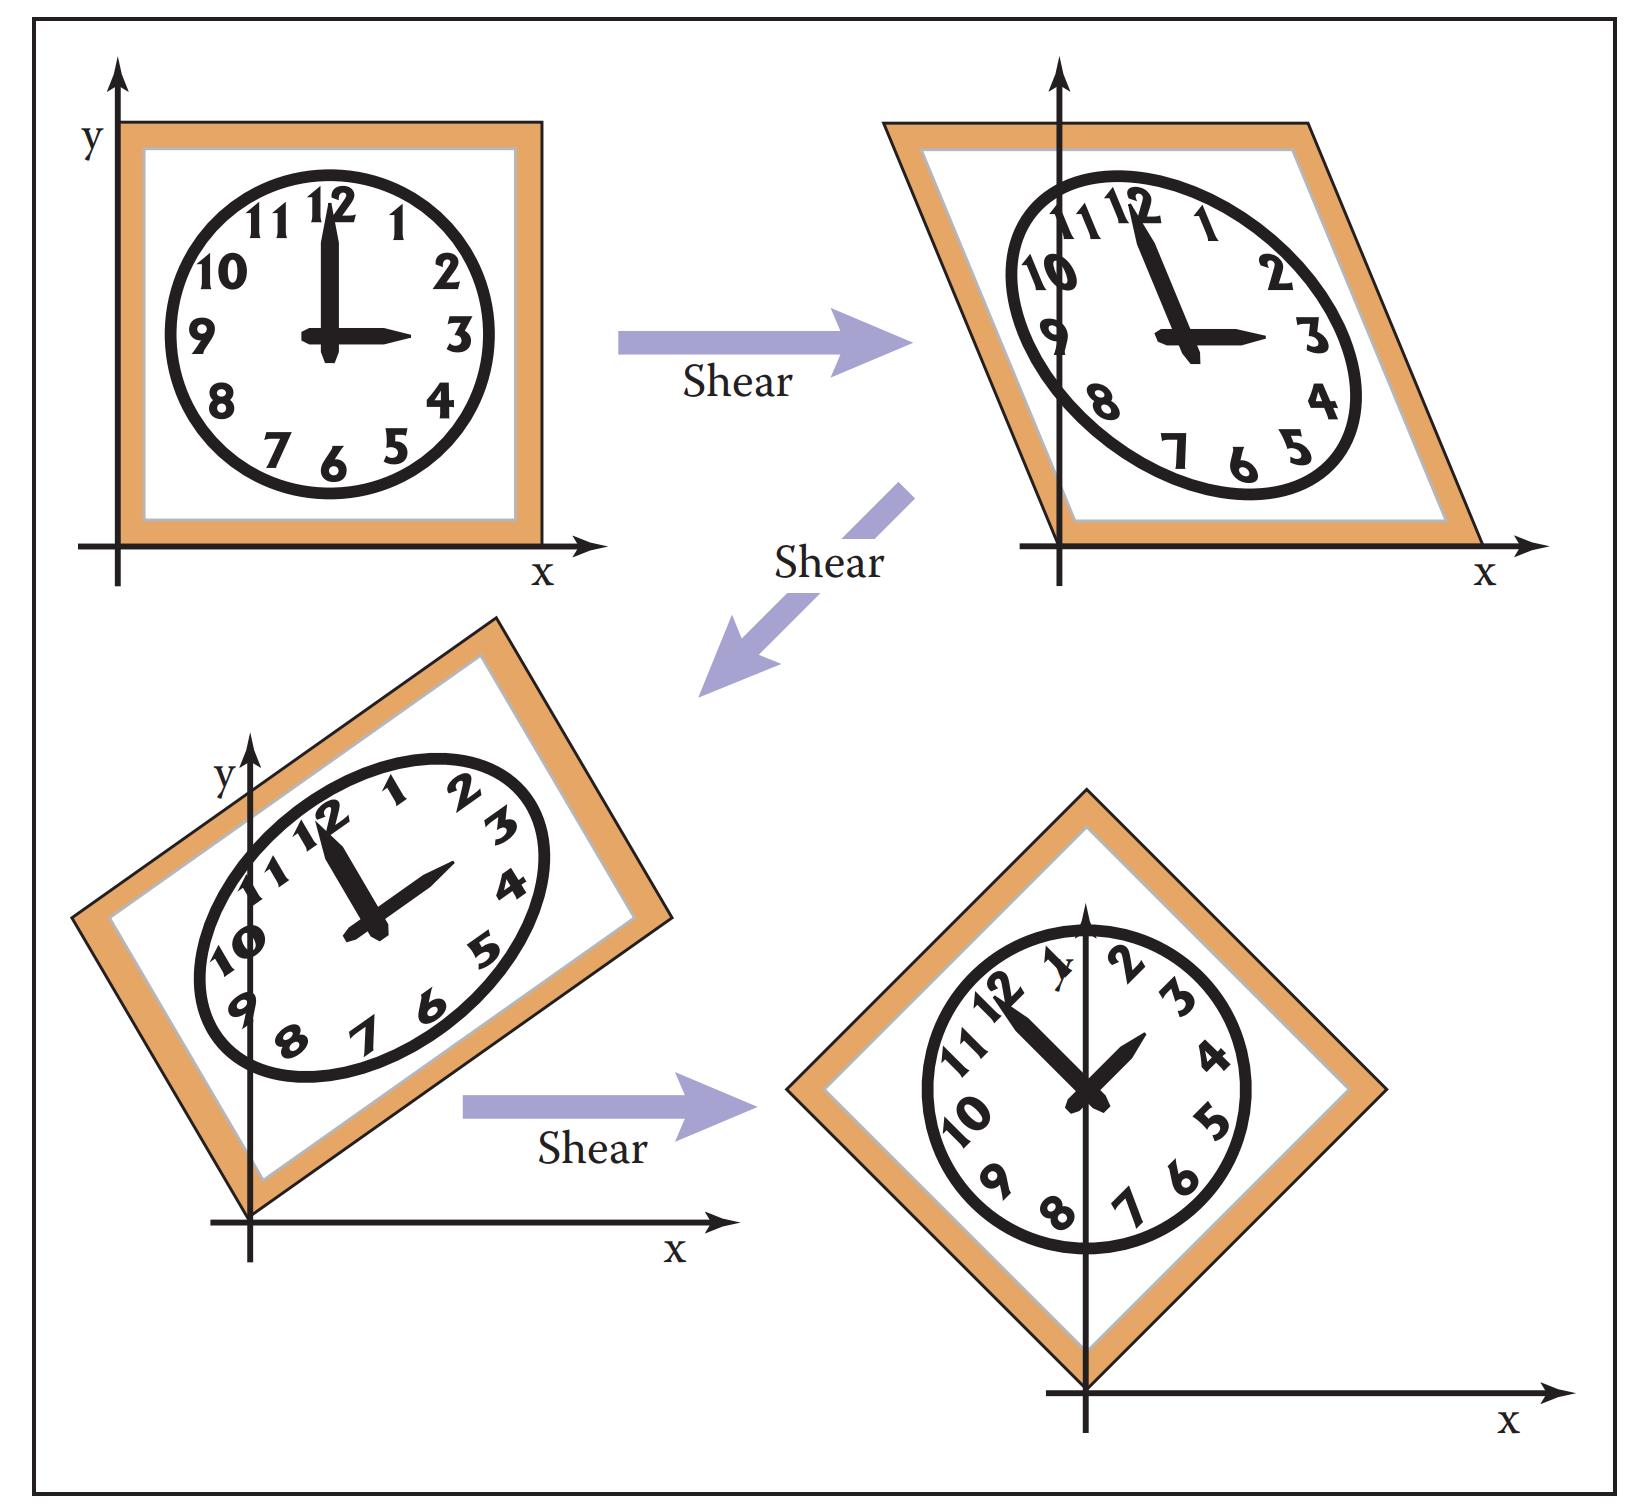
\includegraphics[scale=0.45]{Figure7.15.png}
	\caption{任何二维旋转都可以通过三个剪切变换序列完成。在这种情况下,旋转$45^{\circ}$可以按照式\ref{con:7.2}进行分解。}
	\label{fig:7.15}
\end{figure}	

如果我们把$sj$四舍五入到最近的整数,这就相当于把图像中的每一行都向侧面移动了一定数量的栅格-其中每一行移动的栅格数量都不同。因为每一行的位移都是一样的,这就使得我们在旋转的过程中不会出现空隙。类似的操作也适用于垂直剪切。如此,我们可以很容易地实现一个简单的光栅旋转。

\section{三维线性变换(3D Linear Transformations)}

三维线性变换是二维变换的扩展。例如,沿笛卡尔轴的缩放为:

\begin{equation}
	\operatorname{scale}\left(s_x, s_y, s_z\right)=\left[\begin{array}{ccc}
		s_x & 0 & 0 \\
		0 & s_y & 0 \\
		0 & 0 & s_z
	\end{array}\right]
\nonumber
\end{equation}


